%#BIBTEX latexmk
%#! latexmk IAB_DYNAMICO_kernels
\documentclass[a4paper,twoside,openright]{report}
% \title{{\vspace{2cm}{\Large IcoAtmosBenchmark \\ DYNAMICO kernels} }}
% \author{{\vspace{2cm}{SPPEXA/AIMES Benchmarking team}}}
\title{{{\Large IcoAtmosBenchmark \\ DYNAMICO kernels} }}
\author{{{SPPEXA/AIMES Benchmarking team}}}
\date{\today}
\RequirePackage[l2tabu, orthodox]{nag}

\usepackage[pdftex]{graphicx}
\usepackage[pdftex,usenames,dvipsnames]{color}
\usepackage[pdftex,pdfusetitle]{hyperref}
\usepackage[stretch=30,shrink=20]{microtype}
% \usepackage{times}
% \usepackage{bookman}
% \usepackage{lmodern}
 \usepackage{tgtermes}
\usepackage[T1]{fontenc}
\usepackage{amsmath}
% \usepackage{ascmac}
\usepackage{bm}
% \usepackage{alltt}
\usepackage[round]{natbib}
\usepackage{tabularx}
\usepackage{color}
\usepackage{colortbl}
\usepackage{fancybox}
\usepackage{url}
\usepackage{xspace}
\usepackage{lscape}
\usepackage{listings}
\usepackage[section]{placeins}
\usepackage{flafter}
\usepackage{siunitx}
\usepackage{subcaption}
% \usepackage{pxjahyper}
\hypersetup{% options for hyperref
 bookmarksopen=true,
 bookmarksnumbered=true,
 bookmarksdepth=subsubsection,
 colorlinks=true,
% linkcolor=red,
 linkcolor=Blue,
 citecolor=Brown,
 urlcolor=Red,
}



\usepackage[top=30mm,bottom=35mm,left=30mm,right=30mm]{geometry}
\setcounter{tocdepth}{3}
\setcounter{secnumdepth}{3}
\renewcommand{\thesubsubsection}{(\arabic{subsubsection})}
\renewcommand{\thefootnote}{*\arabic{footnote})}

%Model Names
\newcommand{\IAB}{{IcoAtmosBenchmark }}
\newcommand{\NICAM}{\textsl{NICAM}\xspace}
\newcommand{\DYNAMICO}{\textsl{DYNAMICO}\xspace}
\newcommand{\ICON}{\textsl{ICON}\xspace}

\newcommand{\Item}[1]{~\\\noindent{\bf \large \underline{#1}}\\}

%%%%%%%%%%%%%%%%%%%%%%%%%%%%%%%%%%%%%%%%%%%%%%%%%%%%%%%%%%%%%%%%%%%%%%%%
% source list
%%%%%%%%%%%%%%%%%%%%%%%%%%%%%%%%%%%%%%%%%%%%%%%%%%%%%%%%%%%%%%%%%%%%%%%%
\renewcommand{\lstlistingname}{List}
% \renewcommand{\lstlistlistingname}{リスト目次}
% \renewcommand{\lstlistoflistings}{\begingroup
%   \renewcommand{\lstlistingname}{リスト目次}
%   \tocfile{\lstlistingname}{lol}
% \endgroup}

%%%
\definecolor{darkgreen}{rgb}{0.0, 0.2, 0.13}


\lstloadlanguages{XML,[90]Fortran,perl,c,python,bash,csh}
\definecolor{lstbgcolor} {gray}{0.95}

%%% default style
\lstset{%
numberstyle=\tiny,%
basicstyle=\scriptsize\ttfamily,%
keywordstyle={\color{blue}},%
commentstyle={\slshape\color[named]{Brown}},%
columns=[l]{fullflexible},%
% breaklines=true,breakatwhitespace=true,
% prebreak=\raisebox{0ex}[0ex][0ex]{\ensuremath{\color{red}\hookleftarrow\space}},
aboveskip=2\medskipamount,belowskip=2\medskipamount,%
backgroundcolor={\color{lstbgcolor}},%
frame=single,framerule=0pt,%
framexleftmargin=2pt,framexrightmargin=2pt,framesep=5pt,
numbers=none}

\lstdefinelanguage{NCL}{
sensitive=true,%
morekeywords={load,do,if,else,end,system,print,then,.not.,delete},%
morestring=[b]",%"
stringstyle=\color{darkgreen},%
morecomment=[l]{;}
}

\lstdefinestyle{XML}{language=XML,%
keywordstyle=\color{Maroon},%
tagstyle=\color{DarkBlue},%
usekeywordsintag=true,%
%markfirstintag=true,%
morestring=*[b]",%"
alsoletter={\#},
stringstyle=\color{darkgreen},%
morecomment=[s][\slshape\color{gray}]{<?}{?>},%
morecomment=[n][\slshape\color{gray}]{<!--}{-->},%
commentstyle=\slshape\color{gray},%
emphstyle=\itshape,
breaklines=true,breakatwhitespace=true,%
}

\lstdefinestyle{F90}{%
language=[90]Fortran,%
columns=fixed, basewidth=.44em,%
stringstyle=\color{darkgreen},%
xrightmargin=0em, xleftmargin=0em,%
numbers=left,%
showlines=true,%
deletekeywords={data} }

\lstdefinestyle{Bash}{%
language=bash,%
deletekeywords={go,true}}

\lstdefinestyle{Csh}{%
language=csh,%
deletekeywords={go,true}}

\lstdefinestyle{Python}{%
language=python}

\lstdefinestyle{Ncl}{%
language=NCL}

%%% for XML script
\lstnewenvironment{LstXML}[1][]%
{\lstset{style=Xml,#1}}{}

%%% for F90 source
\lstnewenvironment{LstF90}[1][]%
{\lstset{style=F90,#1}}{}

%%% for Bash script
\lstnewenvironment{LstBash}[1][]%
{\lstset{style=Bash,#1}}{}

%%% for interactive shell
\lstnewenvironment{LstIntSh}[1][]%
{\lstset{style=Bash,language=sh,numbers=none,keywordstyle={},#1}}{}

%%% for (t)csh script
\lstnewenvironment{LstCsh}[1][]%
{\lstset{style=Csh,#1}}{}

%%% for interactive (t)cshell
\lstnewenvironment{LstIntCsh}[1][]%
{\lstset{style=Csh,language=sh,numbers=none,keywordstyle={},#1}}{}

%%% for Python script
\lstnewenvironment{LstPy}[1][]%
{\lstset{style=Python,#1}}{}

\lstnewenvironment{LstNCL}[1][]%
{\lstset{style=Ncl,#1}}{}

%%% For output log
\lstnewenvironment{LstLog}[1][]%
{\lstset{
numbers=none,%
columns=[r]fixed,basewidth=0.45em,%
#1%
}}{}
%%% for inline
\lstMakeShortInline[basicstyle=\normalsize\ttfamily]|


%%%%%%%%%%%%%%%%%%%%%%%%%%%%%%%%%%%%%%%%%%%%%%%%%%%%%%%%%%%%%%%%%%%%%%%%
% misc new commands
%%%%%%%%%%%%%%%%%%%%%%%%%%%%%%%%%%%%%%%%%%%%%%%%%%%%%%%%%%%%%%%%%%%%%%%%

\newcommand{\file}[1]{\path{#1}}

\newcommand{\src}[1]{\texttt{\protect\detokenize{#1}}}

\newcommand{\tool}[1]{\textsf{\protect\detokenize{#1}}}



\newcommand{\TODO}[1]{\fbox{{\Huge \color[named]{Red} #1}}}


\begin{document}
\maketitle
\tableofcontents

\cleardoublepage

\chapter{Brief introduction of DYNAMICO} \label{chap:introdynamico}
\section{\DYNAMICO is}

\DYNAMICO \footnotemark is a new dynamical core for LMD-Z, the atromspheric GCM part
of IPSL-CM Earth System Model.
%
\DYNAMICO is funded by the Indo-French Centre for the Promotion of
Advanced Research, by IPSL and by the G8 Research Councils Initiative on
Multilateral Research Funding, project ICOMEX.


\footnotetext{
This section is based on the \DYNAMICO Wiki page (\url{http://forge.ipsl.fr/dynamico/wiki})
}



The primary goal of \DYNAMICO is to re-formulate in LMD-Z the horizontal
advection and dynamics on a icosahedral grid, while preserving or
improving their qualities with respect to accuracy, conservation laws
and wave dispersion.
%
A broader goal is to revisit all fundamental features of the dynamical
core, especially the shallow-atmosphere/traditional approximation, the
vertical coordinate and the coupling with physics.
%
Also efficient implementation of present and future supercomputing
architectures is a key issue.

This manual describes the overview of \DYNAMICO and each kernel program
briefly.
%
For the details of \DYNAMICO, see
\cite{gmd-8-3131-2015},
etc.


Kernel programs for \DYNAMICO are taken from \DYNAMICO ver 1.0, r339.
%
Main feature of \DYNAMICO-1.0 are;
\begin{itemize}
 \item hydrostatic, traditional shallow atmosphere,
 \item icosahedral-hexagonal C-grid in horizontal, mass-based Lorentz
       staggering in vertical,
 \item Mimetic finite difference + slope-limited finite volume
       transport, and
 \item explicit Runge-Kutta time stepping.
\end{itemize}



\section{Governing equations}

Basic scheme of \DYNAMICO is the energy/voticity conserving schemes and
the curl (vector-invariant) form.
%
To deliver governing equations, \DYNAMICO adopts the Hamiltonian
formulation of the equations of motion.
%
This Hamiltonian theory has been extended for compressible hydrostatic
flows and for non-Eulerian vertical coordinates \citep{JAS-D-13-0339,MWR-D-14-00069}.
%
Derivation of governing equations is complicated, we skip it here. See
\cite{gmd-8-3131-2015} etc.




\section{Horizontal and vertical grid}

\DYNAMICO adopts the icosahedral-hexagonal C-grid in horizontal and
mass-based Lorentz staggering grid in vertical.
%
\autoref{f:ico_c_grid} shows horizontal and vertical grids.

Scalar variables, such as entropy $\Theta$, are defined on the center of
hexagonal control volume (circle points in the figure), velocities and fluxes,
are defined on the edge (square points), and tracer are
defined on the vertex (triangle points).
%
See \cite{gmd-8-3131-2015} for details.


\begin{figure}
 \centering
 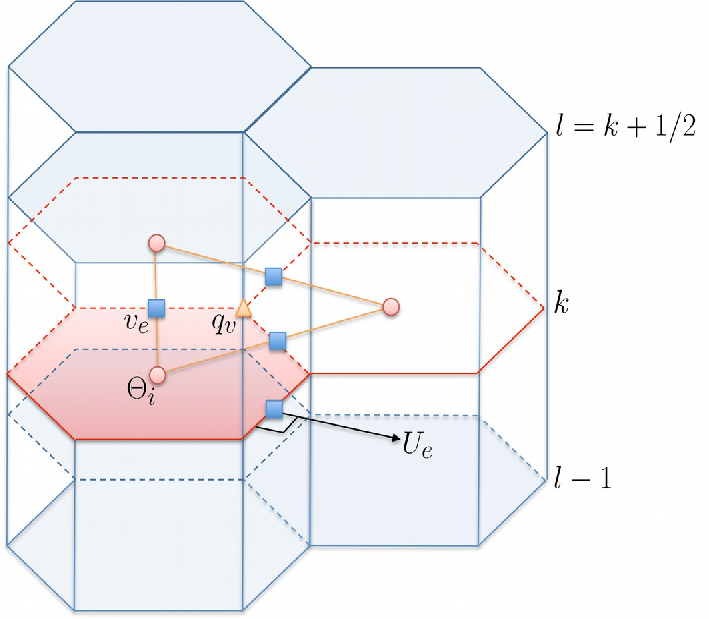
\includegraphics[scale=1]{figs/AIMES_DYNAMICO-08-0.png}
 \caption{Icosahedral C-grid and Lorenz grid.}\label{f:ico_c_grid}
%http://www.lmd.polytechnique.fr/~dubos/Talks/2014DubosAGU.pdf
\end{figure}



\section{Parallelization}

Like \NICAM and \DYNAMICO, icosahedral grids on entire globe can be
separated by 10 ``diamonds'', each are consist of neighboring two
triangles of an icosahedron.
%
Each diamonds can be divided in \src{nsplit_i}$\times$\src{nsplit_j} areas,
and one of divided area,
called ``patch'' in \DYNAMICO, is the basis of domain decomposition.
%
\src{nsplit_i} and \src{nsplit_j} are control parameter and read from
configuration file on execution.
%
One MPI process can handle \src{ndomain} patches, which is decided by
the number of total patchs and the number of MPI processes.



\section{Data structure}\label{s:data_structure}

Basic data structure in \DYNAMICO is a \src{t_field}, as shown in
\autoref{l:t_field}.
%
One instance of \src{t_field} is to access one field within one patch.
%
One MPI process may handle several patches, and one field may be usually
an array of \src{t_field}.
%
Allocation and halo-exchange routines are work on \src{t_field(:)}
variables, and other high-level computational routines work on them, too.
%
See the next section as an example.

\begin{LstF90}[%
caption={\src{t_field} structure},%
label={l:t_field}%
]
  TYPE t_field
    CHARACTER(30)      :: name
    REAL(rstd),POINTER :: rval2d(:)
    REAL(rstd),POINTER :: rval3d(:,:)
    REAL(rstd),POINTER :: rval4d(:,:,:)

    INTEGER,POINTER :: ival2d(:)
    INTEGER,POINTER :: ival3d(:,:)
    INTEGER,POINTER :: ival4d(:,:,:)

    LOGICAL,POINTER :: lval2d(:)
    LOGICAL,POINTER :: lval3d(:,:)
    LOGICAL,POINTER :: lval4d(:,:,:)

    INTEGER :: ndim
    INTEGER :: field_type
    INTEGER :: data_type
    INTEGER :: dim3
    INTEGER :: dim4
  END TYPE t_field
\end{LstF90}

One of members of \src{t_field} are pointer to the array of
\src{REAL(rstd)}, \src{INTEGER} or \src{LOGICAL}, and whose dimension is
one, two or three.
%
If the field is horizontal, such as surface pressure or sea surface
temperature, \src{rval2d} is used.
%
Note that horizontal index $I$ and $J$ are merged to one dimension.


\autoref{f:aimes_dynamico-30-0} shows horizontal indexing in \DYNAMICO.
%
As shown in previous chapter, \DYNAMICO adopts icosahedral grid, and
control volume is hexagonal as usual.
%
One ``patch'' is rhomboid, and can be indexed as two-dimensional, each
size are \src{iim} and \src{jjm}, as shown in left figure of
\autoref{f:aimes_dynamico-30-0}.
%
These can be re-written as usual orthogonal i-j plane, shown in the
right figure of \autoref{f:aimes_dynamico-30-0}.
%
The \src{n} point in the figure is surrounded by
six neighbouring cells, named \src{right}, \src{rup}, etc.
%
So stencil calculation comes from finite difference in horizontal uses
seven points, not five as in usual orthogonal grid.

\begin{figure}[htpb]
\centering
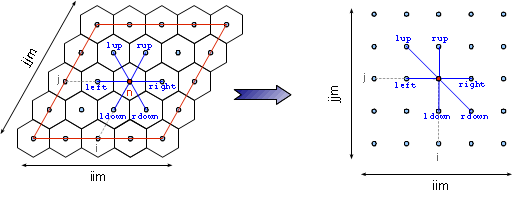
\includegraphics[scale=0.7]{figs/AIMES_DYNAMICO-30-0.png}
\caption{Horizontal indexing}\label{f:aimes_dynamico-30-0}
\end{figure}

The number of the edge point is three times larger than that of the center point.
As shown in \autoref{f:rel_center_edge}, each center point manages three edge points.
These points are named \src{u_right}, \src{u_lup}, and \src{u_ldown}.

\begin{figure}[htpb]
\centering
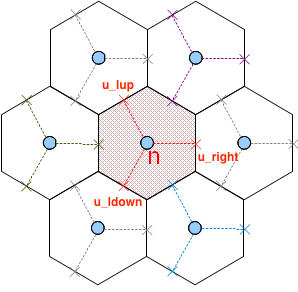
\includegraphics[scale=0.5]{figs/AIMES_DYNAMICO-30-1.png}
\caption{Relationship of center points and edge points}\label{f:rel_center_edge}
\end{figure}

To allocate one \src{t_field} instance, subroutine \src{allocate_field}
is called.
%
Below is the example of allocating orography named ``phis''.

\begin{LstF90}
 ! Time-independant orography
    CALL allocate_field(f_phis,field_t,type_real,name='phis')
\end{LstF90}



\section{Code structure}

Global program structure of \DYNAMICO is as follows.

In the main program, after the various initialization, time step loop is
carried by a single subroutine \src{timeloop}.
%
\autoref{f:pad_timeloop} shows PAD (Problem Analysis
Diagram)\footnotemark of main processes in subroutine \src{timeloop}.
%
As seen in the top of this PAD,

\footnotetext{See \autoref{s:pad} for reading PAD.}

\begin{figure}[htb]
 \centering
 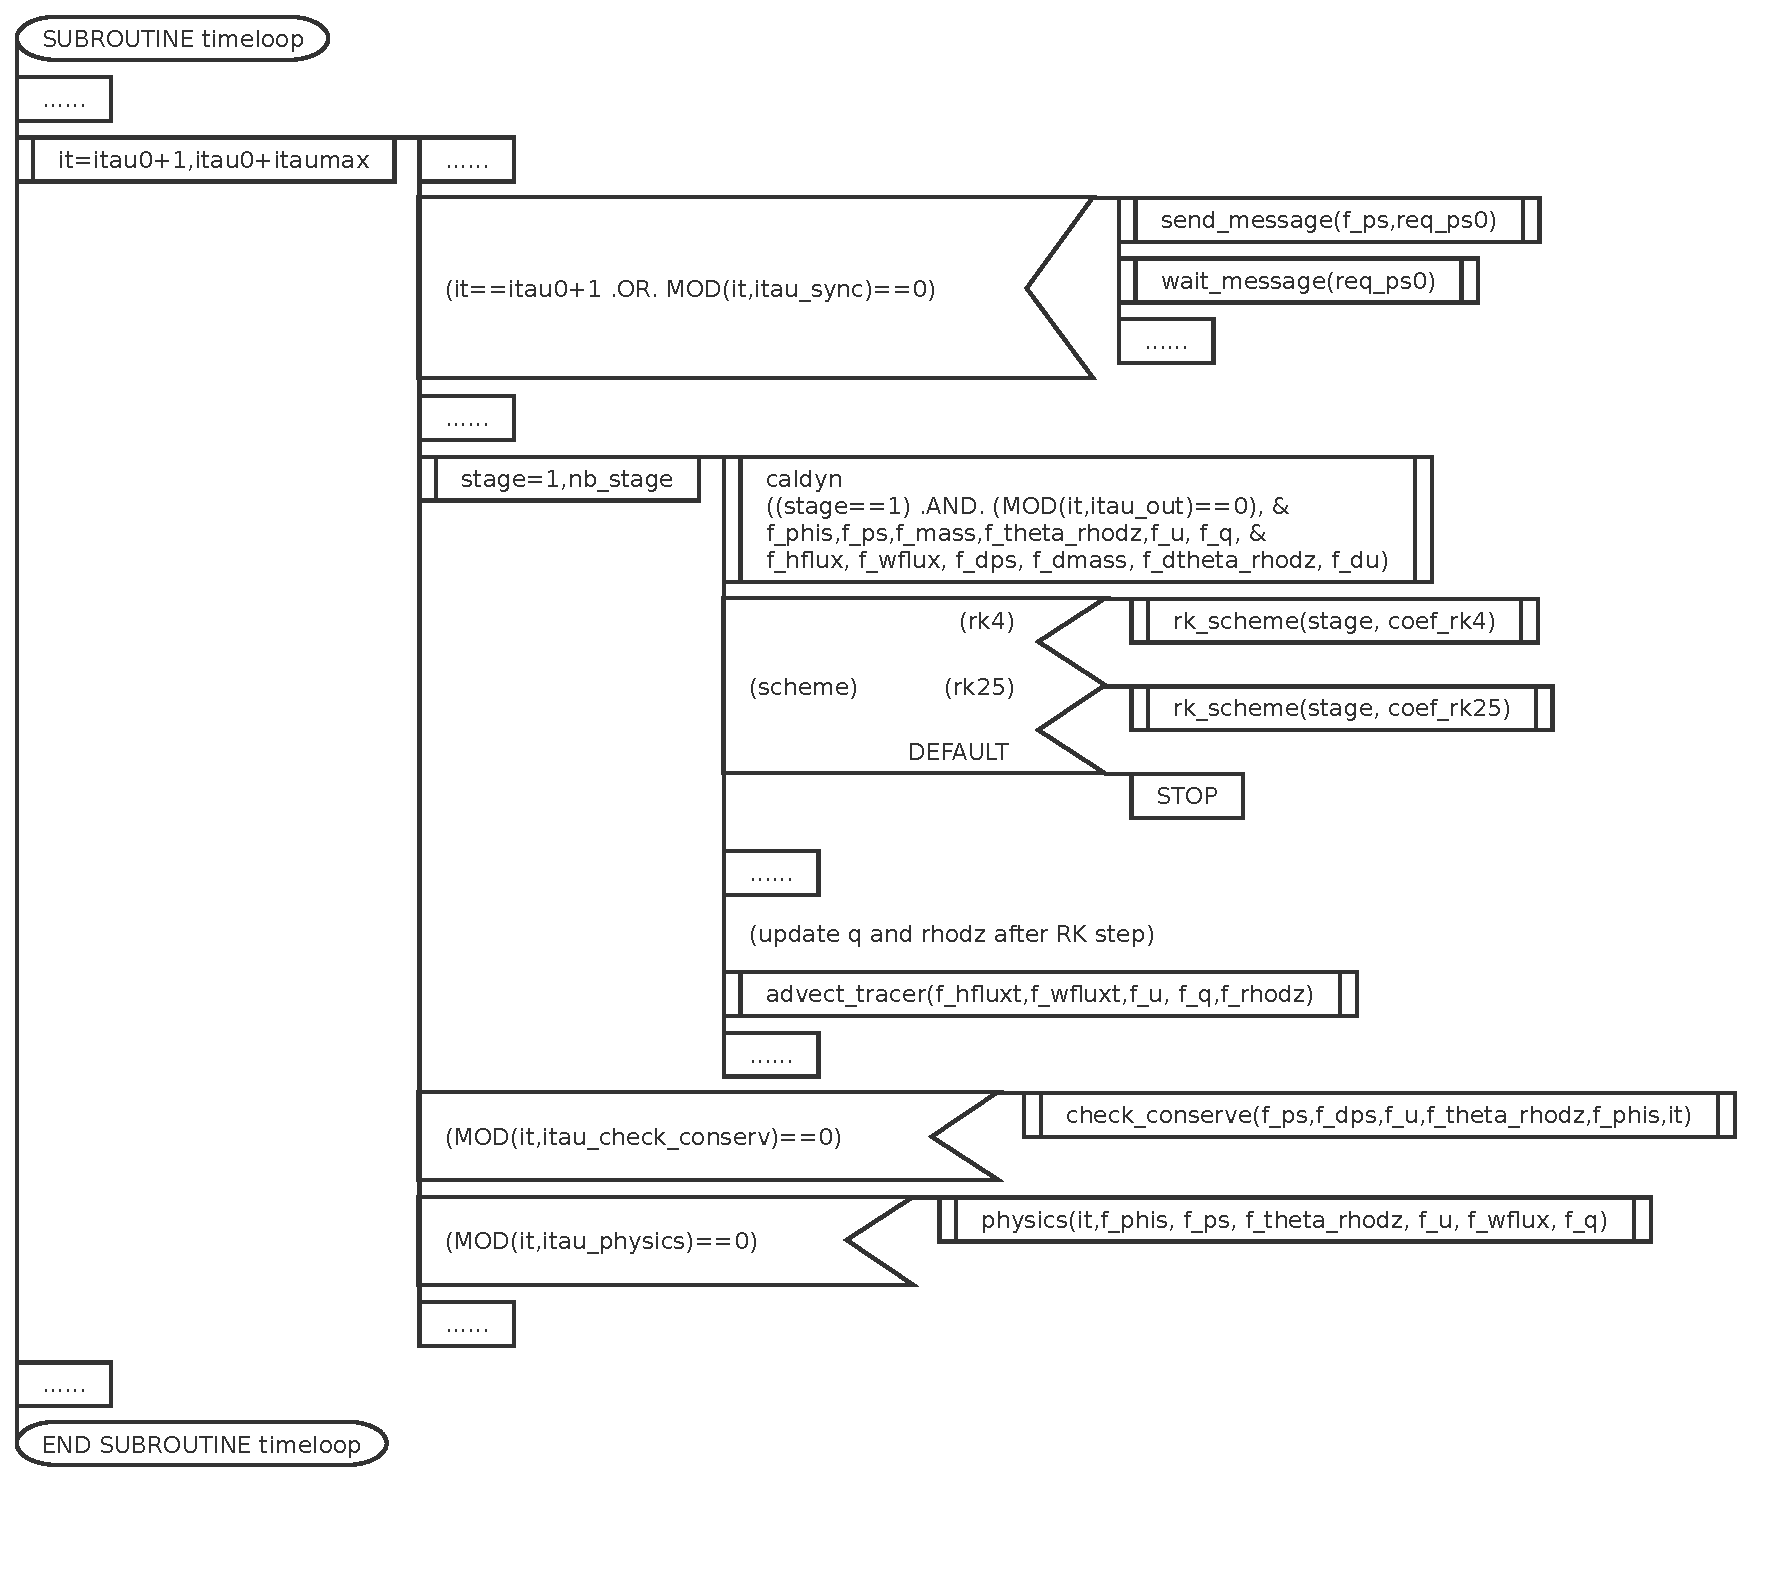
\includegraphics[scale=.4]{figs/timeloop.pdf}
 \caption{PAD of \src{timeloop}}\label{f:pad_timeloop}
\end{figure}

Main time step loop is described in first \src{it} loop, from step
\src{itau0} to \src{itau0+italmax}.
%
First IF block in this loop is for halo exchange of several fields,
using subroutine \src{send_message} and \src{wait_message}.
%
In the next \src{stage} loop subroutine \src{caldyn}, one of
\src{*_scheme} and \src{advect_tracer} are called sequentially.
%
Subroutine \src{caldyn} calculate dynamical terms such as potential
vorticity, etc.
%
Subroutine \src{*_scheme} is for time-advancing. For example,
\src{rk_scheme} uses Runge-Kutta scheme.
%
This is a default scheme for this kernel package.
%
Subroutine \src{advect_tracer} is to calculate advection of tracer
quantities.
%
Here variable \src{nb_stage} in the loop range is the number of
iteration necessary for each time-advancing scheme. For example,
\src{nb_stage=1} for Euler scheme, \src{nb_stage=4} for Runge-Kutta scheme.
%
Finally, if time step \src{it} is at \src{itau_physics}'th step,
subroutine \src{physics} is called to calculate physics part.



\autoref{l:definition_caldyn} is the definition part of subroutine
\src{caldyn}\footnotemark,
and \autoref{f:pad_caldyn} is the PAD of it.
%
\footnotetext{Here is the version in \file{caldyn_gcm.f90}}
%
Note that all of current four kernel program in this package is taken
from the subroutine called from this \src{caldyn} (See \autoref{s:kernelize}).
%
As mentioned in \autoref{s:data_structure}, all of fields used in this
subroutine is given as pointers of instance of \src{t_field}.

\begin{LstF90}[%
caption={Definition part of \src{caldyn}},%
label={l:definition_caldyn}%
]
  SUBROUTINE caldyn(write_out,f_phis, f_ps, f_mass, f_theta_rhodz, f_u, f_q, &
       f_hflux, f_wflux, f_dps, f_dmass, f_dtheta_rhodz, f_du)
    USE icosa
    USE disvert_mod, ONLY : caldyn_eta, eta_mass
    USE vorticity_mod
    USE kinetic_mod
    USE theta2theta_rhodz_mod
    USE wind_mod
    USE mpipara
    USE trace
    USE omp_para
    USE output_field_mod
    USE checksum_mod
    IMPLICIT NONE
    LOGICAL,INTENT(IN)    :: write_out
    TYPE(t_field),POINTER :: f_phis(:)
    TYPE(t_field),POINTER :: f_ps(:)
    TYPE(t_field),POINTER :: f_mass(:)
    TYPE(t_field),POINTER :: f_theta_rhodz(:)
    TYPE(t_field),POINTER :: f_u(:)
    TYPE(t_field),POINTER :: f_q(:)
    TYPE(t_field),POINTER :: f_hflux(:), f_wflux(:)
    TYPE(t_field),POINTER :: f_dps(:)
    TYPE(t_field),POINTER :: f_dmass(:)
    TYPE(t_field),POINTER :: f_dtheta_rhodz(:)
    TYPE(t_field),POINTER :: f_du(:)

    REAL(rstd),POINTER :: ps(:), dps(:)
    REAL(rstd),POINTER :: mass(:,:), theta_rhodz(:,:), dtheta_rhodz(:,:)
    REAL(rstd),POINTER :: u(:,:), du(:,:), hflux(:,:), wflux(:,:)
    REAL(rstd),POINTER :: qu(:,:)
    REAL(rstd),POINTER :: qv(:,:)

! temporary shared variable
    REAL(rstd),POINTER  :: theta(:,:)
    REAL(rstd),POINTER  :: pk(:,:)
    REAL(rstd),POINTER  :: geopot(:,:)
    REAL(rstd),POINTER  :: convm(:,:)
    REAL(rstd),POINTER  :: wwuu(:,:)

    INTEGER :: ind
    LOGICAL,SAVE :: first=.TRUE.
\end{LstF90}

\begin{figure}[htb]
\centering
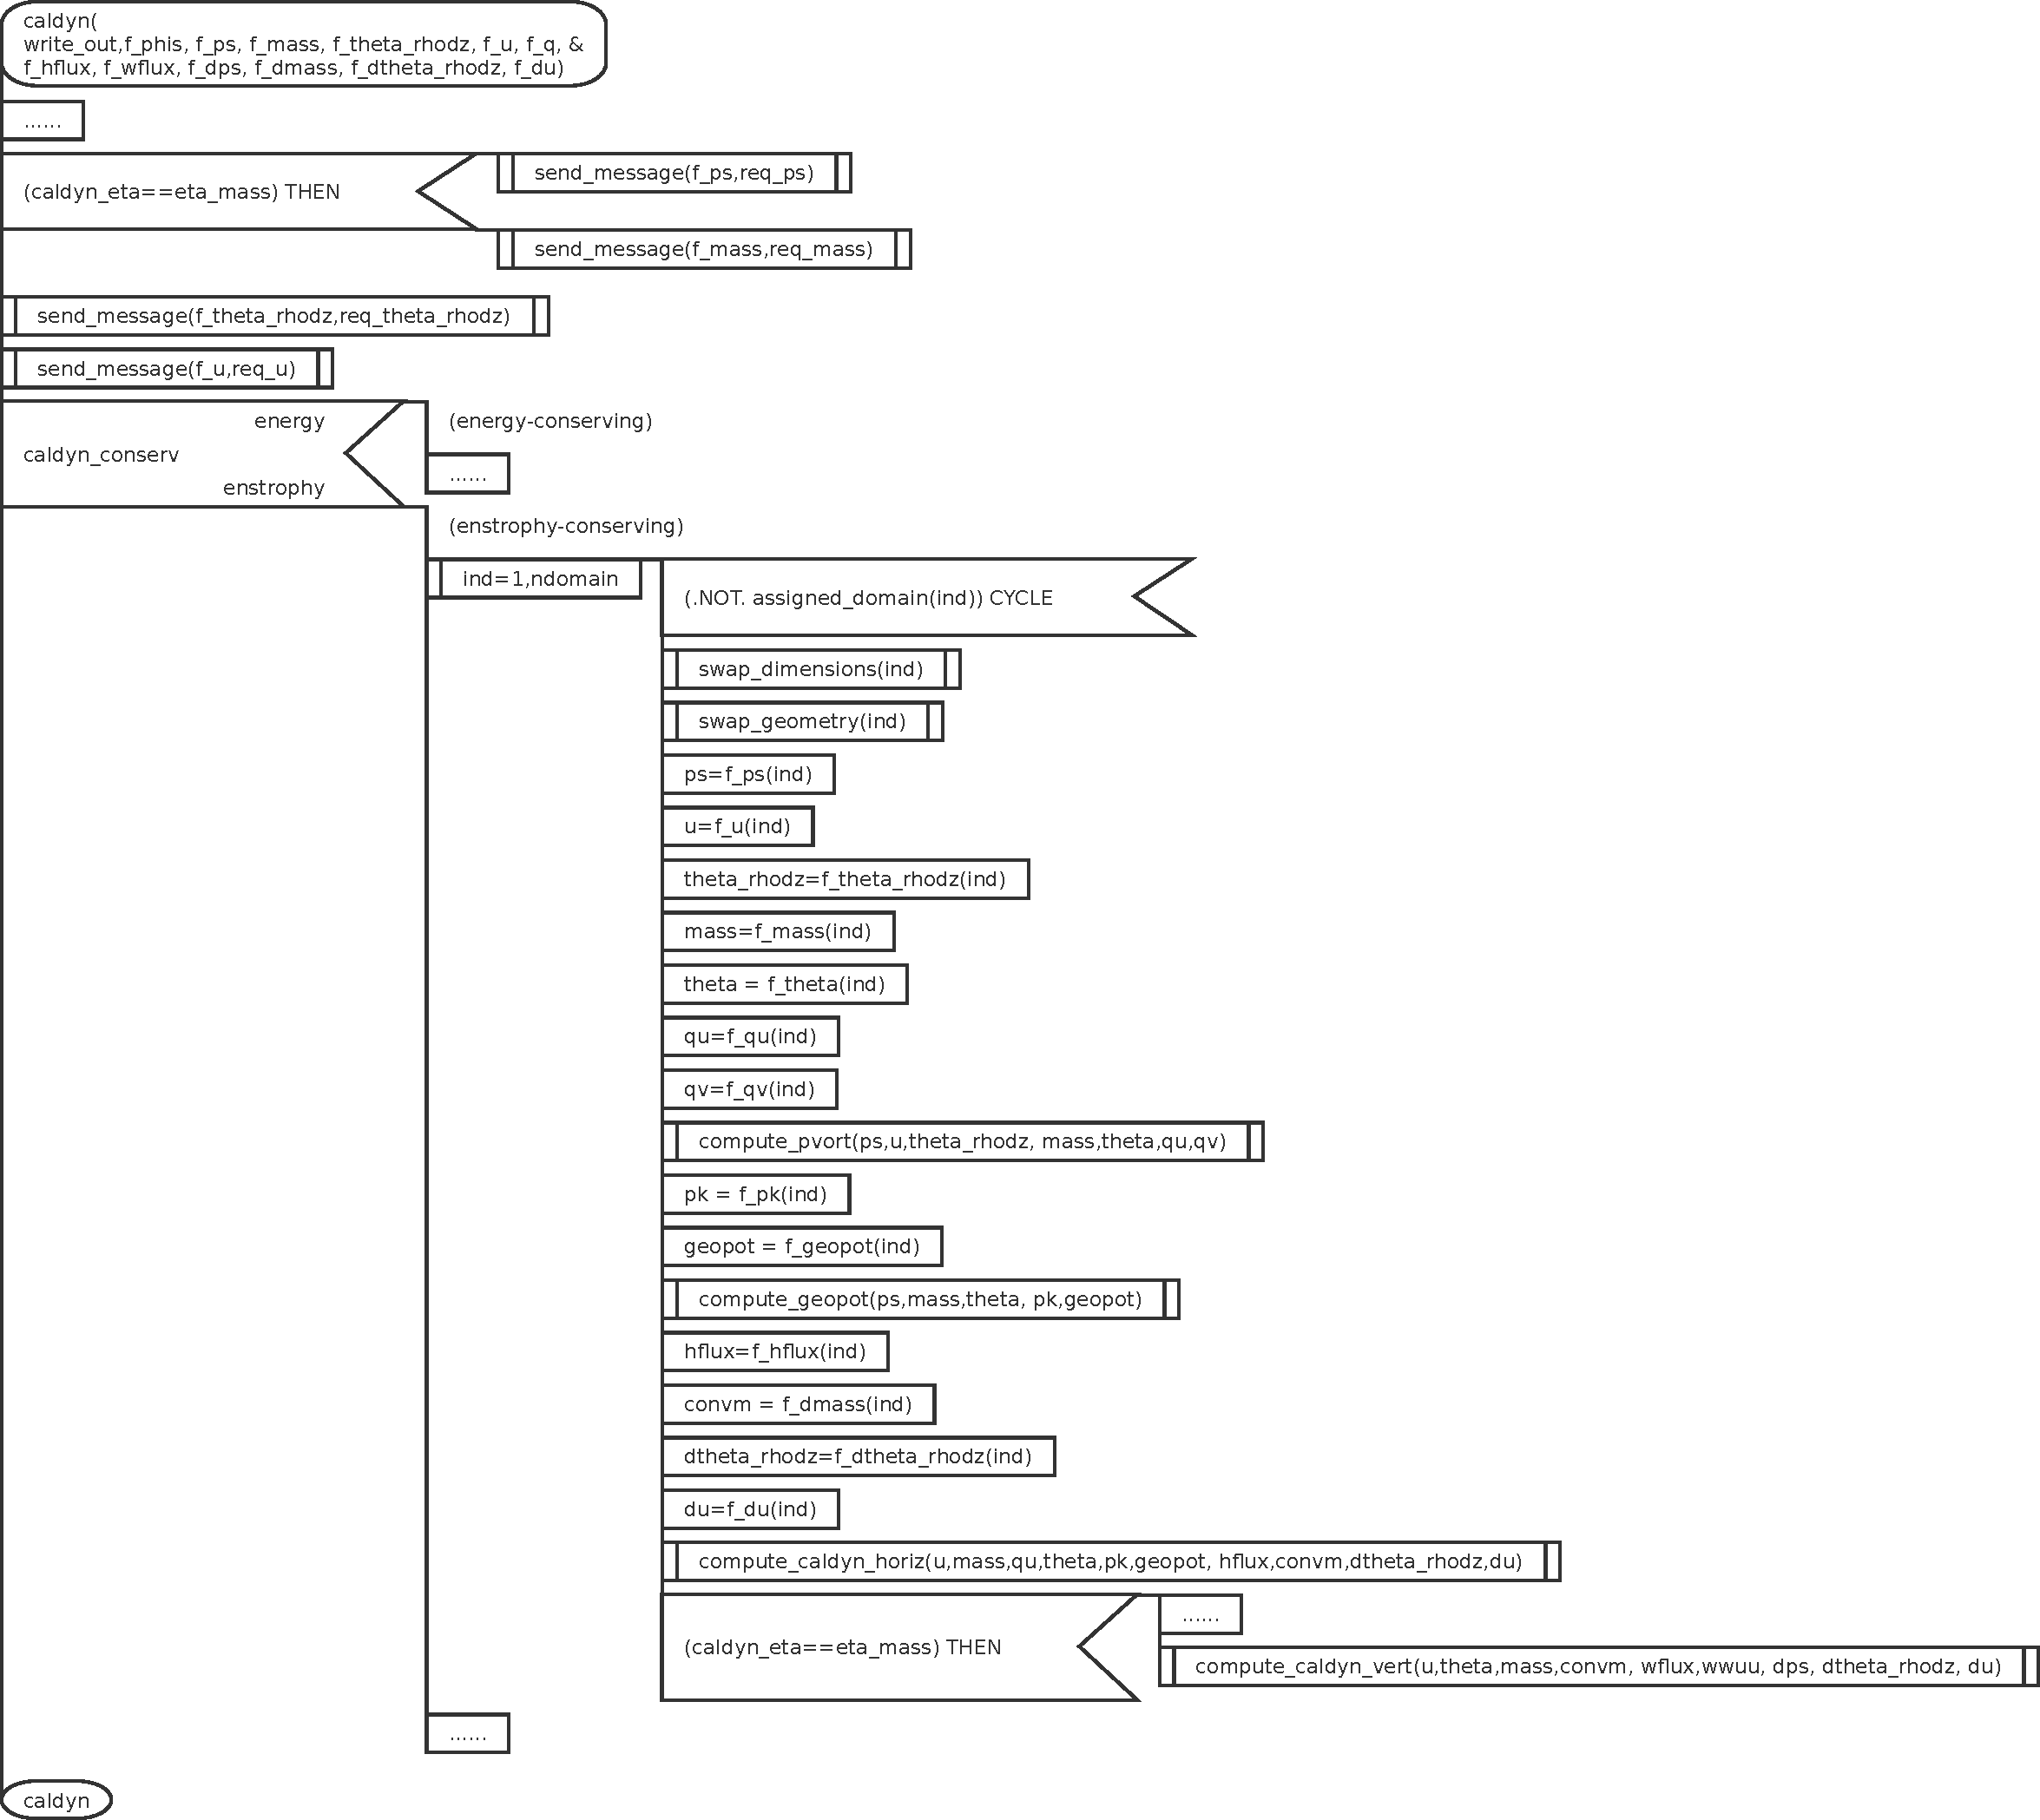
\includegraphics[scale=.4]{figs/caldyn.pdf}
\caption{PAD of \src{caldyn}}\label{f:pad_caldyn}%
\end{figure}

In \autoref{f:pad_caldyn} there are some assignment from
\src{t_field} to real pointer, such as \src{ps = f_ps(ind)}.
%
This is defined as module procedure and generic subroutine
\src{get_val} and using interface assignment.
%
All of them are defined in module \src{field_mod} in \file{field.f90}.


\clearpage

\chapter{Description of each kernel} \label{chap:kerneldynamico}
\section{Overview and common stuff}

\subsection{Kernelize}\label{s:kernelize}


Kernel programs in this package are as follows;
%
\begin{itemize}
 \item \src{comp_pvort}
 \item \src{comp_geopot}
 \item \src{comp_caldyn_horiz}
 \item \src{comp_caldyn_vert}
\end{itemize}
%
All kernels are single subroutines in the original\footnotemark
\DYNAMICO, and extracted and imposed to the wrapper for the kernel program
%
Each subroutine has no modification, except using modules and some
parameter settings.


All of input arrays and most of arrays/variables defined in various
modules in the original model are read from input data file.
%
Input data for each subroutine and reference (output) data are dumped
from the execution of original \DYNAMICO.
%
Main routine of each kernel program reads these input and reference
data, and call the subroutine with them as arguments for 1000 times, in
current setting, then compare output values with reference data.


\footnotetext{
Note that ``original'' here means ``before kernelize'',
since some bug fixes have made by AICS.
Please contact the address shown on the back cover of this manual for details.
}


Kernel programs output several log messages to the standard output, such as:
\begin{itemize}
%\setlength{\itemsep}{0pt}
 \item min/max/sum of input data,
 \item min/max/sum of output data,
 \item min/max/sum of difference between output and validation data,
 \item computational time (elapsed time).
\end{itemize}
%
Elapsed time is measured using \src{omp_get_wtime()}.

There are sample output files for the reference in \src{reference/} directory
of each kernel program, and also they are shown in``Input data and
result'' section of each kernel program in this document.


\subsection{MPI and OpenMP}

While original \DYNAMICO is parallelized by MPI and OpenMP, all kernel
programs in this package are meant to be executed as one process with
no threading.

Different from the \NICAM kernel programss in this package, you don't
need MPI library to compile/execute \DYNAMICO kernel programs, but you
need to make OpenMP enable in order to use \src{omp_get_wtime()}.

\subsection{Mesuring environment}\label{s:measuring_env}

In the following sections, the example of performance result part of the
log output file of each kernel program is shown.
%
These were measured on the machine environment shown in
\autoref{t:machine_env},
with setting \src{export IAB_SYS=Ubuntu-gnu-ompi} on compilation
(See \file{QuickStart.md}).


\begin{table}[htbp]
\centering
\caption{Measuring environment}\label{t:machine_env}
\small
\begin{tabularx}{.8\textwidth}{llX}
\hline
component & specification & notes \\
\hline
 CPU & Xeon E5-2630v4 @2.2GHz (10cores) x2 & HT disabled, TB enabled\\
 Memory & 256GB &\\
 Storage & SSD (SATA) &\\
 OS & Ubuntu 16.04.4 LTS &\\
 Compiler & GNU 5.4.0 & \\
\hline
\end{tabularx}
\end{table}


% \begin{table}
% \centering
% \caption{Measuring environment(Compiler, MPI)}\label{t:machine_env_2}
% \small
% \begin{tabularx}{.9\textwidth}{XXXX}
% \hline
% \src{IAB_SYS} & OS & Compiler & MPI \\
% \hline
% Ubuntu-gnu-ompi  & Ubuntu16.04 & GNU 5.4.0  & OpenMPI 1.10.2\\
% Ubuntu-pgi-ompi  & Ubuntu16.04 & PGI 17.4.0 & OpenMPI 1.10.2\\
% Ubuntu-intel-ompi& Ubuntu16.04 & Intel 2018 & OpenMPI 3.0.0\\
% \hline
% \end{tabularx}
% \end{table}

%#! latexmk -pv IAB_DYNAMICO_kernels
\section{\src{comp_pvort}}

\subsection{Description}

Kernel \src{comp_pvort} is taken from the original subroutine
\src{compute_pvort} in \DYNAMICO.
%
This subroutine is originally defined in module \src{caldyn_gcm_mod}.
%
This module defines subroutine \src{caldyn}, which is the main
subroutines for dynamics part of the model, and several sub-subroutines
for various terms in the governing equation, such as potential
vorticity, geopotential, etc.
%
This subroutine calculates potential vorticity.


\subsection{Discretization and code}

\autoref{l:definition_comp_pvort} shows the definition part of this subroutine
and \autoref{f:pad_comp_pvort} shows the PAD of
this.
%
Note that sources shown here are modified in the process of
kernelization from the original distributed version.

\begin{LstF90}[%
caption={Definition part of \src{compute_pvort}},%
label={l:definition_comp_pvort}%
]
SUBROUTINE compute_pvort(ps,u,theta_rhodz, rhodz,theta,qu,qv)
  USE icosa
  USE disvert_mod, ONLY : mass_dak, mass_dbk, caldyn_eta, eta_mass
  USE exner_mod
  USE trace
  USE omp_para
  IMPLICIT NONE
  REAL(rstd),INTENT(IN)  :: u(iim*3*jjm,llm)
  REAL(rstd),INTENT(IN)  :: ps(iim*jjm)
  REAL(rstd),INTENT(IN)  :: theta_rhodz(iim*jjm,llm)
  REAL(rstd),INTENT(INOUT) :: rhodz(iim*jjm,llm)
  REAL(rstd),INTENT(INOUT) :: theta(iim*jjm,llm)
  REAL(rstd),INTENT(INOUT) :: qu(iim*3*jjm,llm)
  REAL(rstd),INTENT(INOUT) :: qv(iim*2*jjm,llm)

  INTEGER :: i,j,ij,l
  REAL(rstd) :: etav,hv, m
\end{LstF90}
%
Here \src{u}, \src{ps}, \src{theta_rhodz} are velocity on the edge, surface pressure,
and mass-weighted potential temperature, respectively.
Output arrays \src{rhodz}, \src{theta}, \src{qu}, \src{qv} are mass, potential temperature,
potential vorticity on the edge, and potential vorticity on the vertex, respectively.
%
These arrays except \src{ps} have two dimensions, first one is for
horizontal index and second one is for vertical index.
%
Note that \DYNAMICO adopts C-grid in horizontal, number of horizontal
grid point for scalar, or number of control volume, in one domain is
\src{iim*jjm}, but \src{u} and \src{qu} are defined on the edge of
control volume, the size of the first dimension of them are
\src{iim*3*jjm}.  Also \src{qv} is defined on the vertex of control
volume, the size of the first dimension of \src{qv} is \src{iim*2*jjm}.

\begin{figure}[htbp]
 \centering
 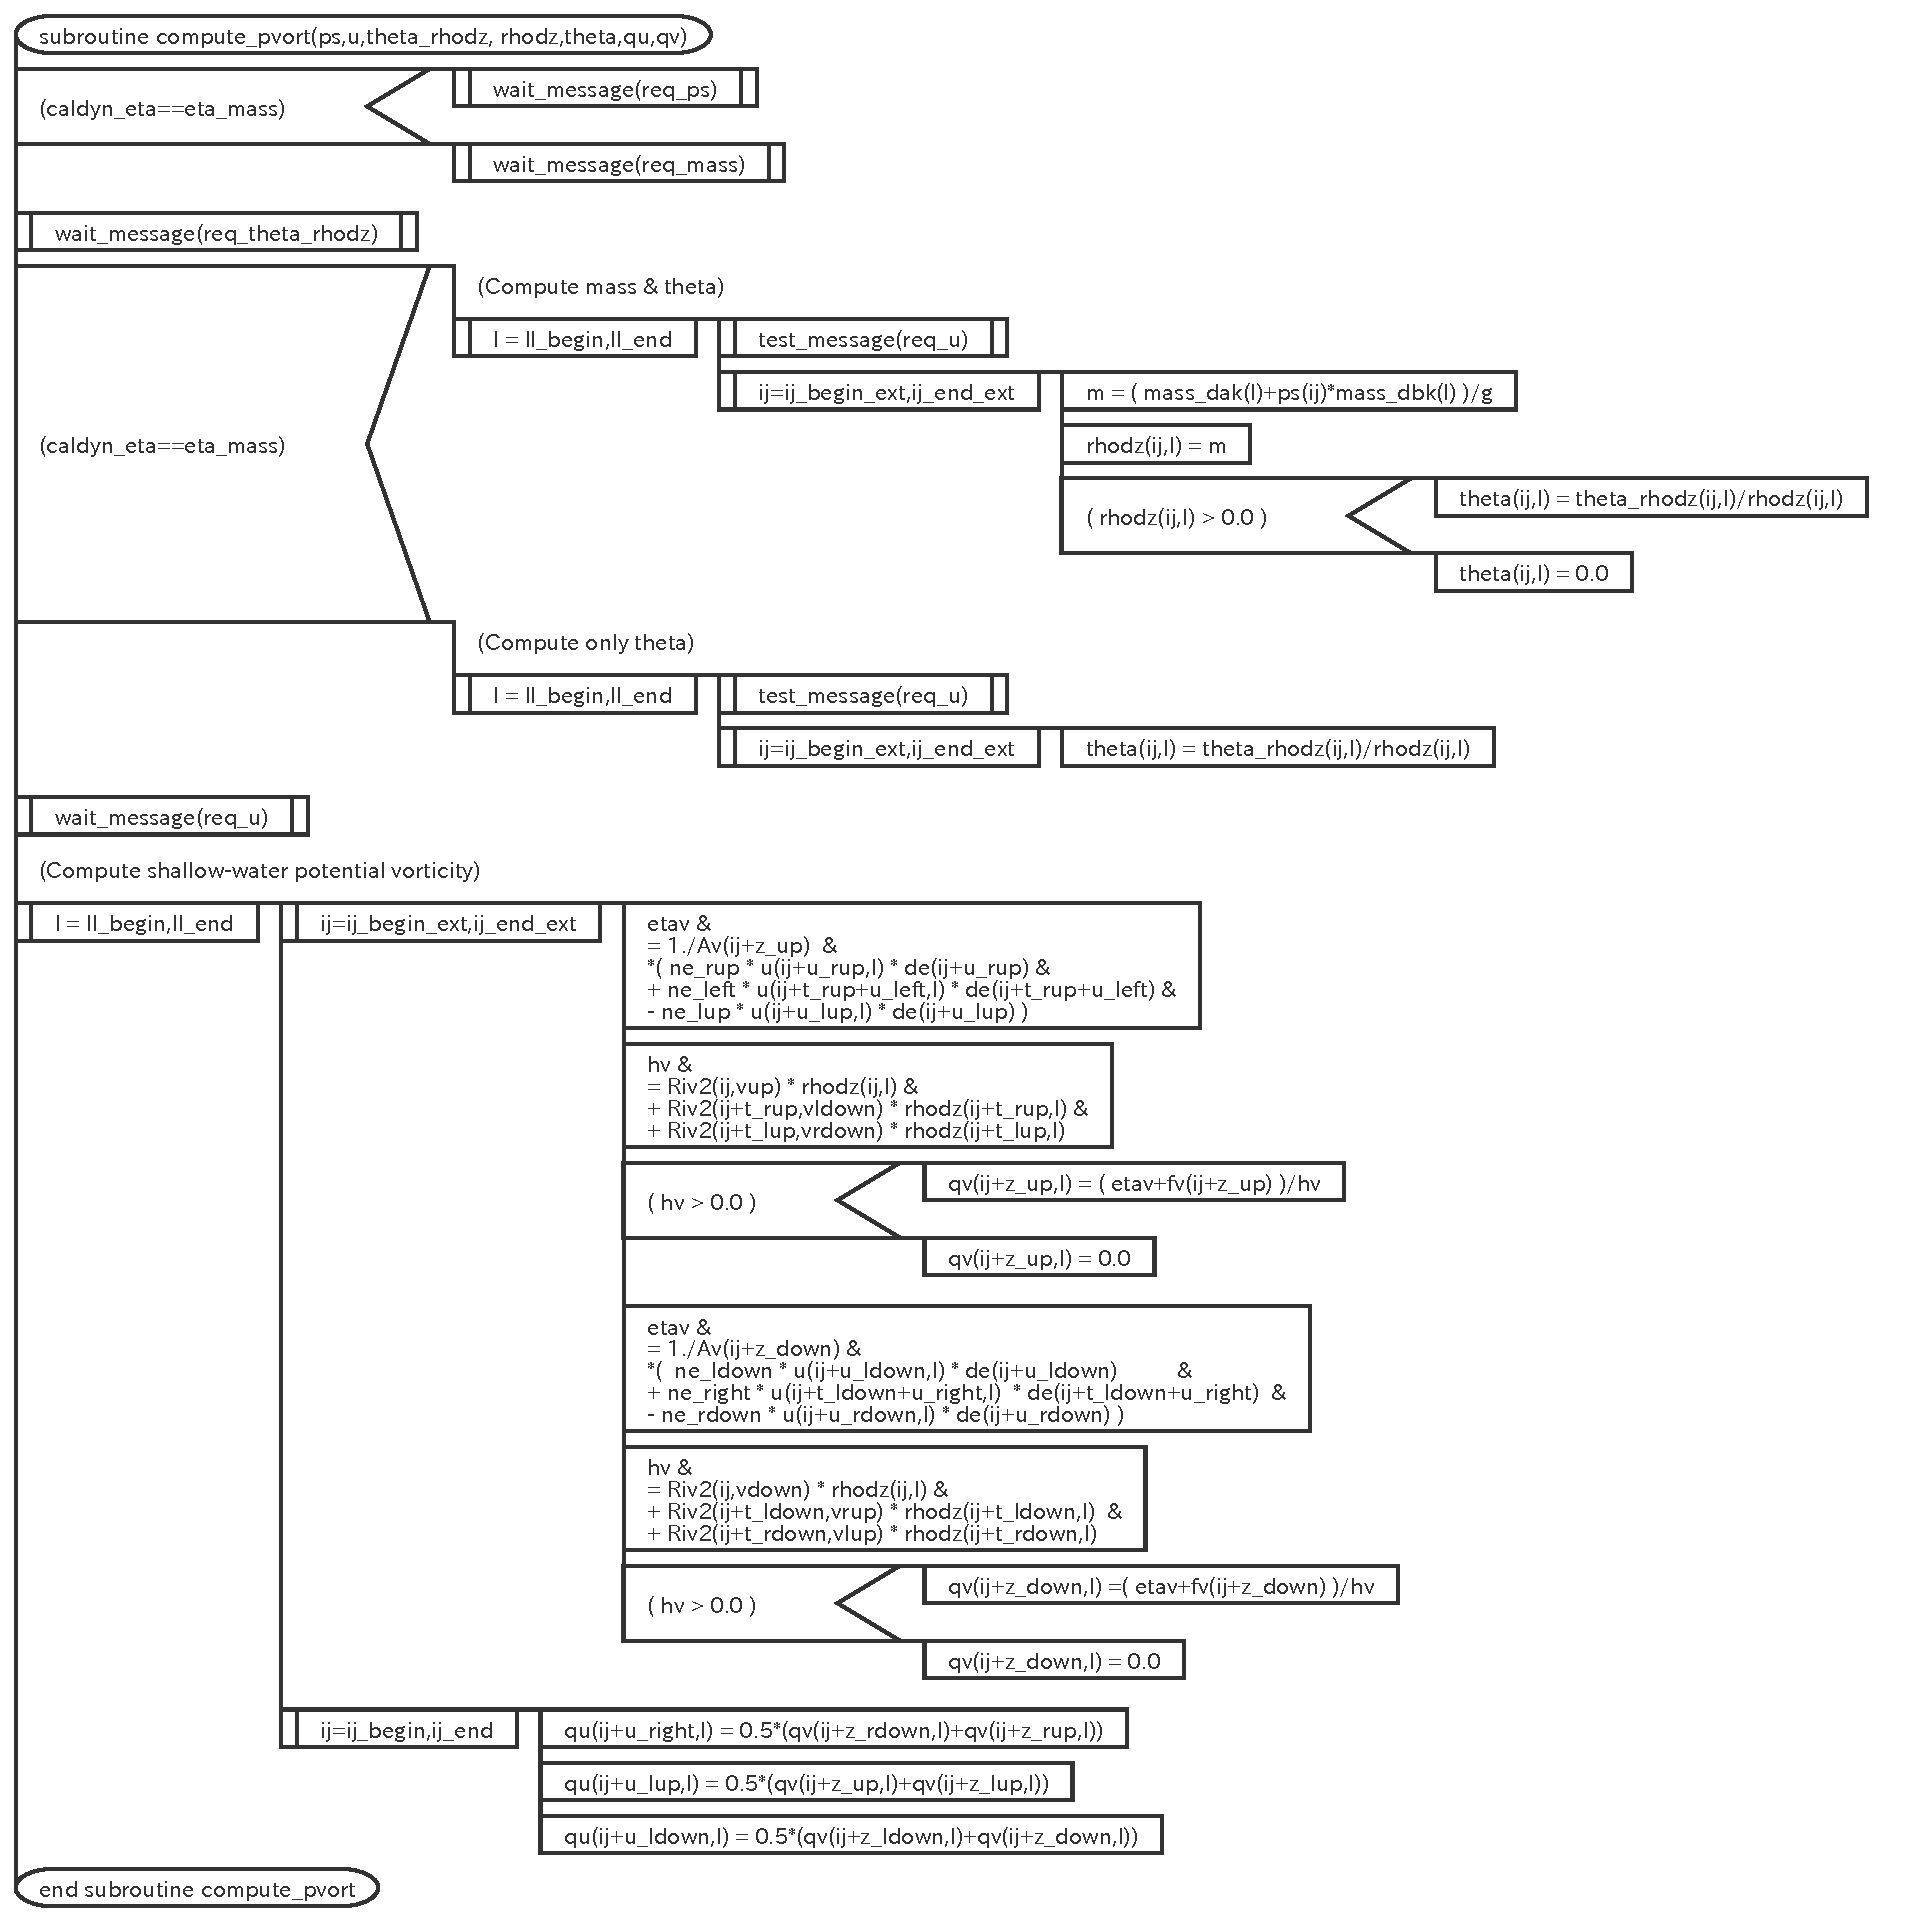
\includegraphics[scale=.4]{figs/pvort.pdf}
 \caption{PAD of \src{compute_pvort}}\label{f:pad_comp_pvort}%
\end{figure}

The first section of this subroutine calculates \src{theta} in the
double loop of \src{ij} and \src{l}.
%
Note that in this kernel package, \src{caldyn_eta} is set as
\src{eta_mass}, that means that vertical coordinate $\eta$ uses
Lagrangian vertical coordinate, rather than mass coordinate.
%
In the second section, \src{qv} at two points, \src{qv(ij+z_up,l)} and
\src{qv(ij+z_down,l)}, are calculated in the first double loop, then
\src{qu} at three pounts, \src{qu(ij+u_right,l)}, \src{qu(ij+u_lup,l)}
and \src{qu(ij+l_down,l)} are calculated.

\clearpage



\subsection{Input data and result}

Input data file is prepared and you can download from official server using
\file{data/download.sh} script.
%
This data file is created by original \DYNAMICO\footnotemark with
Held-Suarez case parameter set included in the original source archive.
%
\footnotetext{with slight modification by AICS.}
%
Max/min/sum of input/output data of the kernel subroutine are output as
a log.
%
Below is an example of \src{$IAB_SYS=Ubuntu-gnu-ompi} case.

\begin{LstLog}
 [KERNEL] comp_pvort
 *** Start  initialize
                iim, jjm, llm:    23    25    19
             ij_begin, ij_end:    48   528
     ij_begin_ext, ij_end_ext:    24   552
             ll_begin, ll_end:     1    19
        t_right, t_rup, t_lup:     1    23    22
     t_left, t_ldown, t_rdown:    -1   -23   -22
        u_right, u_rup, u_lup:     0  1173   575
     u_left, u_ldown, u_rdown:    -1  1150   553
           z_rup, z_up, z_lup:   598     0   597
     z_ldown, z_down, z_rdown:   -23   575   -22
                   caldyn_eta:     1
                            g:     9.80000000
 +check[Av              ] max=  4.1228713627140027E+11,min=  0.0000000000000000E+00,sum=  3.2428753277257527E+13
 +check[de              ] max=  4.5171816240714993E+06,min=  0.0000000000000000E+00,sum=  4.7785815753077912E+08
 +check[Riv2            ] max=  3.8193271158709069E-01,min=  0.0000000000000000E+00,sum=  9.6499999999999977E+02
 +check[fv              ] max=  8.2383275804860789E-05,min= -6.6879410680009186E-05,sum=  4.1115175112148659E-03
 +check[mass_dak        ] max=  3.9864758943842335E+03,min= -4.2200064724847380E+03,sum=  1.1368683772161603E-13
 +check[mass_dbk        ] max=  1.6280745944237918E-01,min=  0.0000000000000000E+00,sum=  1.0000000000000000E+00
 *** Finish initialize
 *** Start kernel
 ### check point iteration:        1000
 ### Input ###
 +check[u               ] max=  4.1278968179782127E-01,min= -4.1278968179782127E-01,sum=  1.6791131703073393E+01
 +check[ps              ] max=  1.0000000000000000E+05,min=  1.0000000000000000E+05,sum=  5.7500000000000000E+07
 +check[theta_rhodz     ] max=  3.9393370687019045E+05,min=  0.0000000000000000E+00,sum=  1.8099621340626464E+09
 +check[theta_prev      ] max=  8.0139914420291746E+02,min=  0.0000000000000000E+00,sum=  3.8582633571973117E+06
 +check[rhodz_prev      ] max=  1.2306877011993038E+03,min=  0.0000000000000000E+00,sum=  5.3979591836733194E+06
 +check[qu_prev         ] max=  1.0339537867296609E-06,min= -8.4408169682701225E-07,sum=  3.9419811615778674E-04
 +check[qv_prev         ] max=  1.0397552030841796E-06,min= -8.4408169685381862E-07,sum=  2.6984926372303133E-04
 ### Output ###
 +check[theta           ] max=  8.0139914420291746E+02,min=  0.0000000000000000E+00,sum=  3.8582633571973117E+06
 +check[rhodz           ] max=  1.2306877011993038E+03,min=  0.0000000000000000E+00,sum=  5.3979591836733194E+06
 +check[qu              ] max=  1.0626772908333491E-06,min= -8.5290650439776975E-07,sum=  3.9864842567446446E-04
 +check[qv              ] max=  1.0855993800007362E-06,min= -8.9078811385791910E-07,sum=  2.7461310165802981E-04
 ### final iteration:        1000
 ### Validation : grid-by-grid diff ###
 +check[theta           ] max=  0.0000000000000000E+00,min=  0.0000000000000000E+00,sum=  0.0000000000000000E+00
 +check[rhodz           ] max=  0.0000000000000000E+00,min=  0.0000000000000000E+00,sum=  0.0000000000000000E+00
 +check[qu              ] max=  0.0000000000000000E+00,min=  0.0000000000000000E+00,sum=  0.0000000000000000E+00
 +check[qv              ] max=  0.0000000000000000E+00,min=  0.0000000000000000E+00,sum=  0.0000000000000000E+00
 *** Finish kernel
\end{LstLog}

Check the lines below \src{``Validation : grid-by-grid diff''} line,
that shows difference between calculated output array and
pre-calculated reference array.
These should be zero or enough small to be acceptable.
%
There are sample output log files in \file{reference/}
in each kernel program directory, for reference purpose.


\subsection{Sample of performance result}

Here's an example of the performance result part of the log output.
Below is an example executed with the machine environment described in \autoref{s:measuring_env}.
%
Note that in this program kernel part is iterated 1000 times.

\begin{LstLog}
 *** Computational Time Report
 *** ID=001 : MAIN_comp_pvort                  T=     0.248 N=   1000
\end{LstLog}

\section{\src{comp_geopot}}

\subsection{Description}

Kernel \src{comp_geopot} is taken from the original subroutine
\src{compute_geopot} in \DYNAMICO.
%
This subroutine is originally defined in module \src{caldyn_gcm_mod}.
%
This module defines subroutine \src{caldyn}, which is the main
subroutines for dynamics part of the model, and several sub-subroutines
for various terms in the governing equation, such as potential
vorticity, geopotential, etc.
%
This subroutine calculates geopotential.

\subsection{Discretization and code}

\autoref{l:definition_comp_geopot} shows the definition part of this subroutine,
and \autoref{f:pad_comp_geopot} shows the PAD of this.

\begin{LstF90}[%
caption={Definition part of \src{compute_geopot}},%
label={l:definition_comp_geopot}%
]
SUBROUTINE compute_geopot(ps,rhodz,theta, pk,geopot)
USE icosa
USE disvert_mod
USE exner_mod
USE trace
USE omp_para
IMPLICIT NONE
  REAL(rstd),INTENT(INOUT) :: ps(iim*jjm)
  REAL(rstd),INTENT(IN)    :: rhodz(iim*jjm,llm)
  REAL(rstd),INTENT(IN)    :: theta(iim*jjm,llm)    ! potential temperature
  REAL(rstd),INTENT(INOUT) :: pk(iim*jjm,llm)       ! Exner function
  REAL(rstd),INTENT(INOUT) :: geopot(iim*jjm,llm+1) ! geopotential

  INTEGER :: i,j,ij,l
  REAL(rstd) :: p_ik, exner_ik
\end{LstF90}

Where \src{ps}, \src{rhodz},
\src{theta}, \src{pk}, and \src{geopot} are
surface pressure, mass,
potential temperature, Exner function, and geopotential, respectively.
%
These arrays except \src{ps} have two dimensions,  first one is for
horizontal index and second one is for vertical index.
%
All of these are defined in the center of control volume in horizontal,
the size of first dimension is \src{iim*jjm}.
%
Also these except \src{ps} and \src{geopot} are defined in the full
level in vertical, the size of second dimension of these are \src{llm},
while \src{geopot} has the size of \src{llm+1}.

\begin{figure}[p]
\centering
 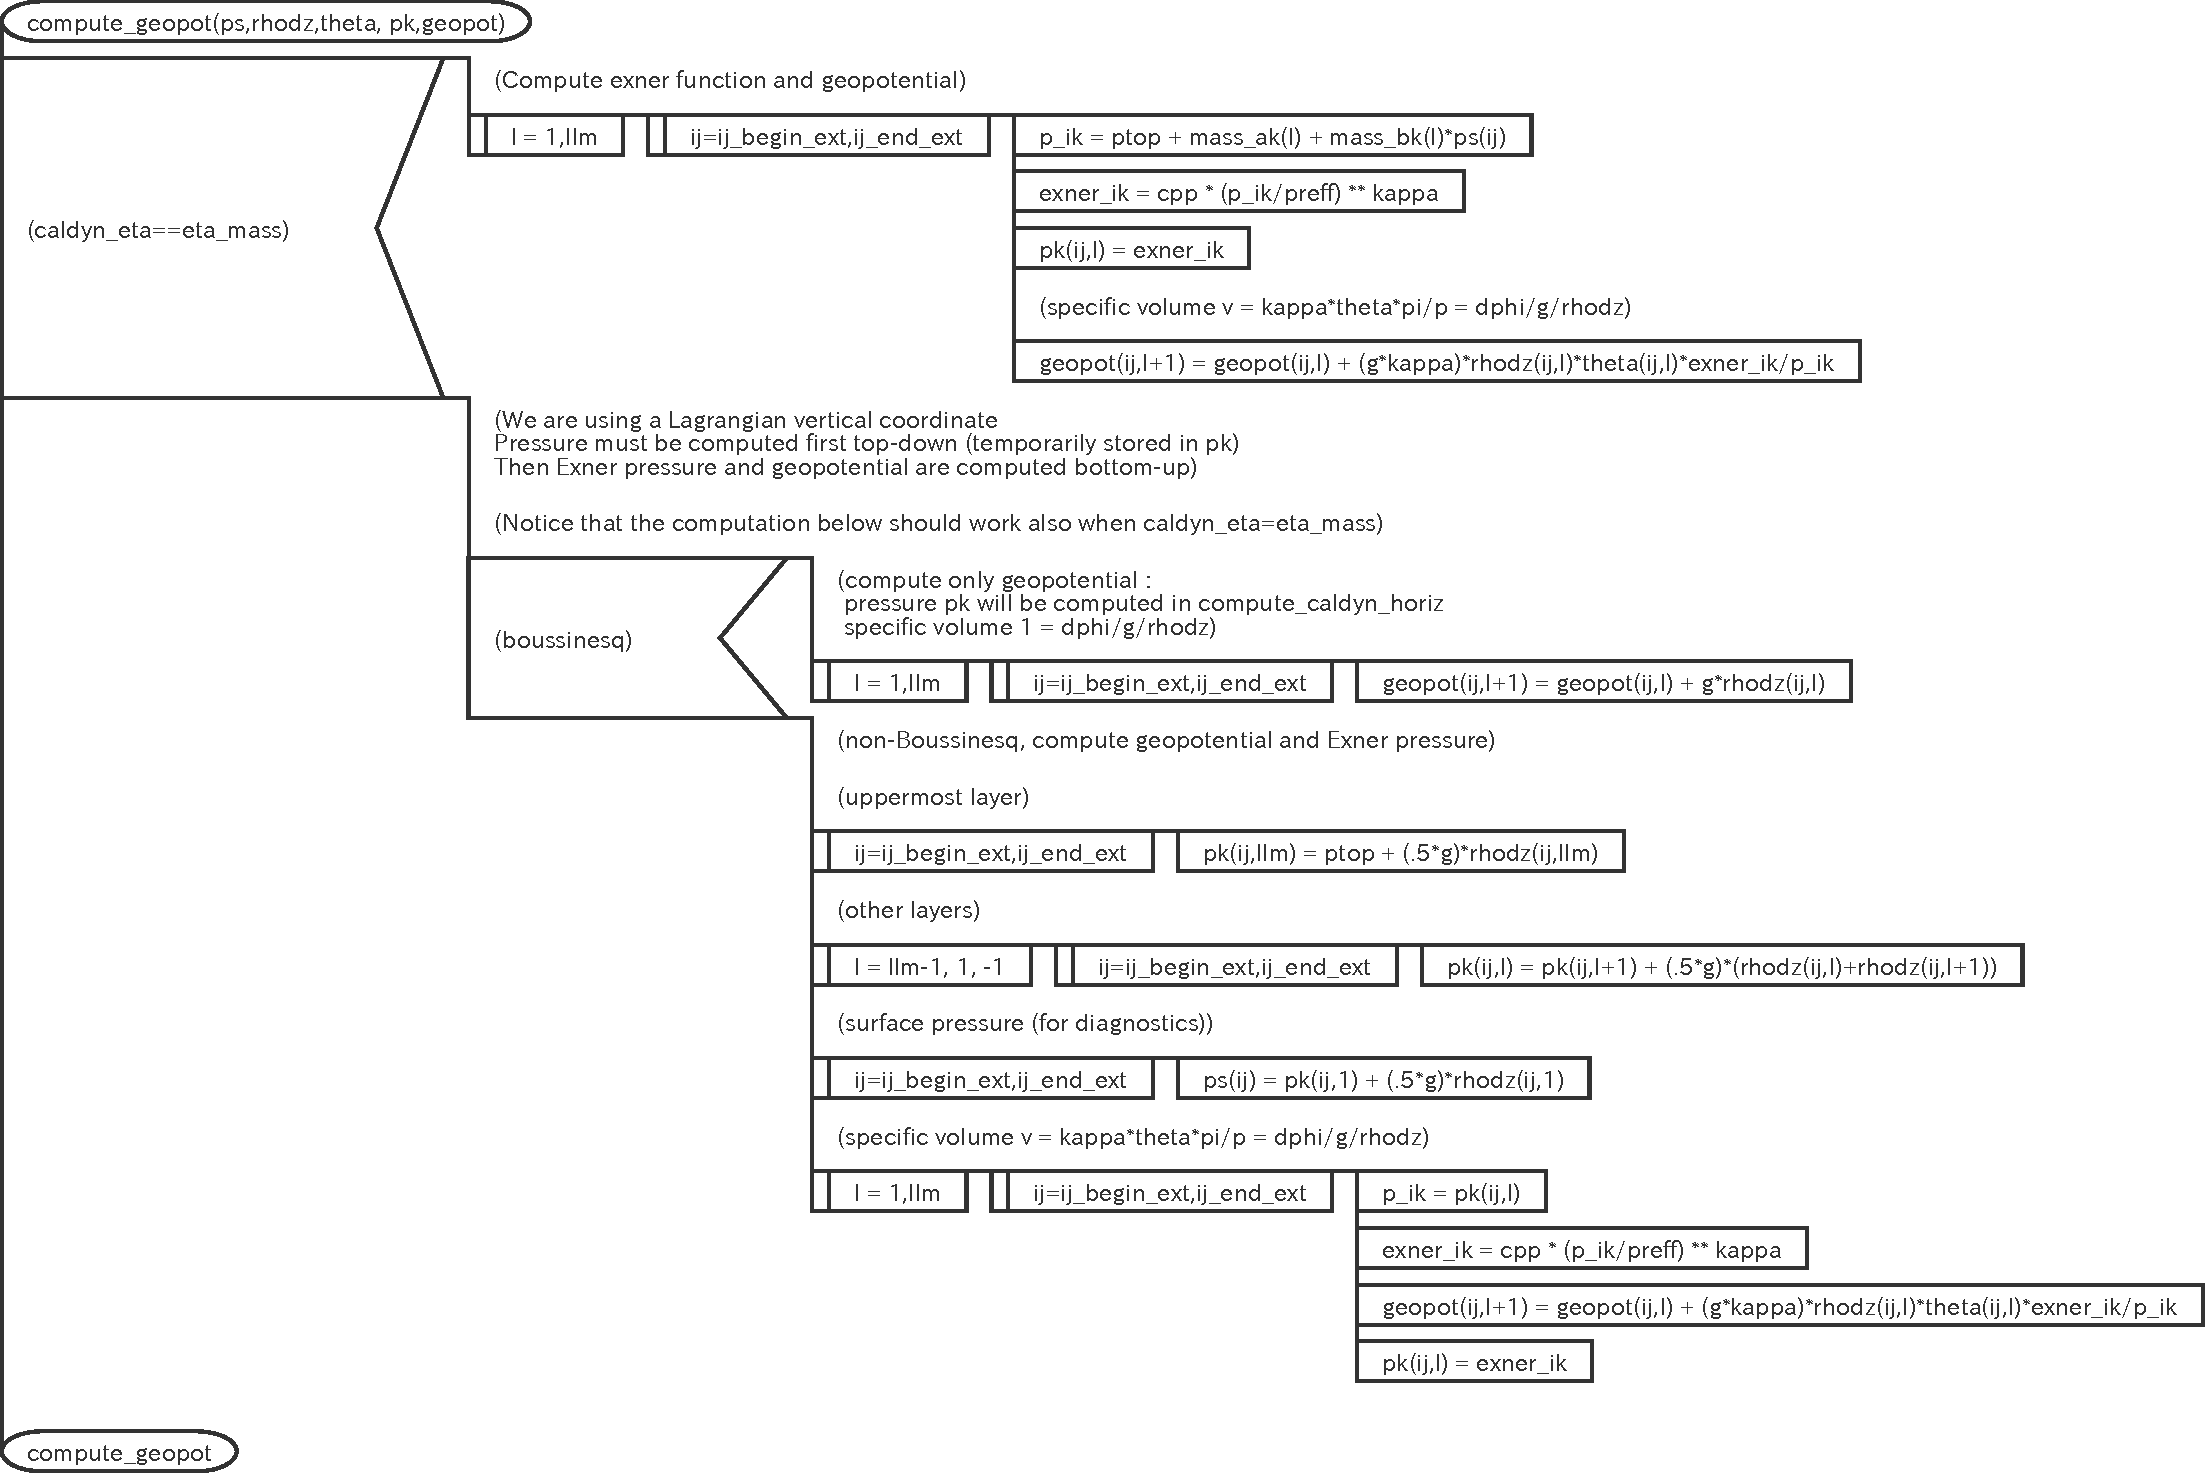
\includegraphics[scale=.45]{figs/geopot.pdf}
 \caption{PAD of \src{compute_geopot}}
 \label{f:pad_comp_geopot}
\end{figure}

Note that in this kernel package
\src{caldyn_eta} is set as \src{eta_mass},
and
\src{boussinesq} is set as \src{.true.},
so in this subroutine only \src{geopot} is calculated as

\begin{LstF90}[numbers=none]
geopot(ij,l+1) = geopot(ij,l) + g*rhodz(ij,l)
\end{LstF90}
%
and Exner pressure
are calculated in subroutine \src{compulte_caldyn_horiz}, which is also
included in this package as kernel \src{comp_caldyn_horiz}.

\clearpage



\subsection{Input data and result}

Input data file is prepared and you can download from official server using
\file{data/download.sh} script.
%
This data file is created by original \DYNAMICO\footnotemark with
Held-Suarez case parameter set included in the original source archive.
%
\footnotetext{with slight modification by AICS.}
%
Max/min/sum of input/output data of the kernel subroutine are output as
a log.
%
Below is an example of \src{$IAB_SYS=Ubuntu-gnu-ompi} case.

\begin{LstLog}
 [KERNEL] comp_geopot
 *** Start  initialize
                iim, jjm, llm:    23    25    19
             ij_begin, ij_end:    48   528
     ij_begin_ext, ij_end_ext:    24   552
             ll_begin, ll_end:     1    19
        t_right, t_rup, t_lup:     1    23    22
     t_left, t_ldown, t_rdown:    -1   -23   -22
        u_right, u_rup, u_lup:     0  1173   575
     u_left, u_ldown, u_rdown:    -1  1150   553
           z_rup, z_up, z_lup:   598     0   597
     z_ldown, z_down, z_rdown:   -23   575   -22
                   caldyn_eta:     1
                   boussinesq:     F
                            g:     9.80000000
 +check[mass_ak         ] max=  2.2205608555404415E+04,min=  2.9655441593806341E+02,sum=  1.7315769223740909E+05
 +check[mass_bk         ] max=  9.8820601234384886E-01,min=  0.0000000000000000E+00,sum=  6.4254510678414123E+00
 *** Finish initialize
 *** Start kernel
 ### check point iteration:        1000
 ### Input ###
 +check[ps_prev         ] max=  1.0000000000000000E+05,min=  1.0000000000000000E+05,sum=  5.7500000000000000E+07
 +check[rhodz           ] max=  1.2306877011993038E+03,min=  0.0000000000000000E+00,sum=  5.3979591836733194E+06
 +check[theta           ] max=  8.0139914420291746E+02,min=  0.0000000000000000E+00,sum=  3.8582633571973117E+06
 +check[pk_prev         ] max=  1.0014594722514462E+03,min=  0.0000000000000000E+00,sum=  6.9872296819747351E+06
 +check[geopot_prev     ] max=  3.8250620498369227E+05,min=  0.0000000000000000E+00,sum=  1.1718001851963627E+09
 ### Output ###
 +check[ps              ] max=  1.0000000000000000E+05,min=  1.0000000000000000E+05,sum=  5.7500000000000000E+07
 +check[pk              ] max=  1.0014594722514462E+03,min=  0.0000000000000000E+00,sum=  6.9872296819747351E+06
 +check[geopot          ] max=  3.8250620498369227E+05,min=  0.0000000000000000E+00,sum=  1.1718001851963627E+09
 ### final iteration:        1000
 ### Validation : grid-by-grid diff ###
 +check[ps              ] max=  0.0000000000000000E+00,min=  0.0000000000000000E+00,sum=  0.0000000000000000E+00
 +check[pk              ] max=  0.0000000000000000E+00,min=  0.0000000000000000E+00,sum=  0.0000000000000000E+00
 +check[geopot          ] max=  0.0000000000000000E+00,min=  0.0000000000000000E+00,sum=  0.0000000000000000E+00
 *** Finish kernel
\end{LstLog}

Check the lines below \src{``Validation : grid-by-grid diff''} line,
that shows difference between calculated output array and
pre-calculated reference array.
These should be zero or enough small to be acceptable.
%
There are sample output log files in \file{reference/}
in each kernel program directory, for reference purpose.

\subsection{Sample of performance result}

Here's an example of the performance result part of the log output.
Below is an example executed with the machine environment described in \autoref{s:measuring_env}.
%
Note that in this program kernel part is iterated 1000 times.

\begin{LstLog}
 *** Computational Time Report
 *** ID=001 : MAIN_comp_geopot                 T=     0.824 N=   1000
\end{LstLog}

\section{\src{comp_caldyn_horiz}}

\subsection{Description}

Kernel \src{comp_caldyn_horiz} is taken from the original subroutine
\src{compute_caldyn_horiz} in \DYNAMICO.
%
This subroutine is originally defined in module \src{caldyn_gcm_mod}.
%
This module defines subroutine \src{caldyn}, which is the main
subroutines for dynamics part of the model, and several sub-subroutines
for various terms in the governing equation, such as potential
vorticity, geopotential, etc.
%
This subroutine calculates several horizontal terms, including mass
flux, Bernouilli term, etc.


\subsection{Discretization and code}

\autoref{l:definition_comp_caldyn_horiz} shows the definition part of this subroutne,
and \autoref{f:pad_comp_caldyn_horiz_1}, \ref{f:pad_comp_caldyn_horiz_2}, \ref{f:pad_comp_caldyn_horiz_3}
show the PAD of this.


\begin{LstF90}[%
caption={Definition part of \src{compute_caldyn_horiz}},%
label={l:definition_comp_caldyn_horiz}%
]
  SUBROUTINE compute_caldyn_horiz(u,rhodz,qu,theta,pk,geopot, hflux,convm, dtheta_rhodz, du)
  USE icosa
  USE disvert_mod
  USE exner_mod
  USE trace
  USE omp_para
  IMPLICIT NONE
    REAL(rstd),INTENT(IN)  :: u(iim*3*jjm,llm)    ! prognostic "velocity"
    REAL(rstd),INTENT(IN)  :: rhodz(iim*jjm,llm)
    REAL(rstd),INTENT(IN)  :: qu(iim*3*jjm,llm)
    REAL(rstd),INTENT(IN)  :: theta(iim*jjm,llm)  ! potential temperature
    REAL(rstd),INTENT(INOUT) :: pk(iim*jjm,llm) ! Exner function
    REAL(rstd),INTENT(IN)  :: geopot(iim*jjm,llm+1)    ! geopotential

    REAL(rstd),INTENT(INOUT) :: hflux(iim*3*jjm,llm) ! hflux in kg/s
    REAL(rstd),INTENT(INOUT) :: convm(iim*jjm,llm)  ! mass flux convergence
    REAL(rstd),INTENT(INOUT) :: dtheta_rhodz(iim*jjm,llm)
    REAL(rstd),INTENT(INOUT) :: du(iim*3*jjm,llm)

    REAL(rstd) :: cor_NT(iim*jjm,llm)  ! NT coriolis force u.(du/dPhi)
    REAL(rstd) :: urel(3*iim*jjm,llm)  ! relative velocity
    REAL(rstd) :: Ftheta(3*iim*jjm,llm) ! theta flux
    REAL(rstd) :: berni(iim*jjm,llm)  ! Bernoulli function

    INTEGER :: i,j,ij,l
    REAL(rstd) :: ww,uu
\end{LstF90}

Where \src{u}, \src{rhodz}, \src{qu}, \src{geopot} are wind velocity on the edge,
mass, potential vorticity on the edge, and geopotential, respectively.
\src{pk}, \src{hflux}, \src{convm}, \src{dtheta_rhodz}, \src{du} are Exner function,
horizontal mass flux on the edge, mass flux convergence,
time derivative of the mass-weighted potential temperature,
and time derivative of wind velocity on the edge.
%
Local arrays \src{cor_NT}, \src{urel}, \src{Ftheta}, \src{berni} are
Coriolis's force, relative velocity, potential temperature flux and
Bernoulli function, respectively.
%
All of these arrays are two dimensional.
%
First dimension is for horizontal index, and the size depends on the point
where the variable is defined, since \DYNAMICO adopts C-grid.
%
Second dimension is for vertical index, and the size is \src{llm},
except \src{llm+1} for \src{geopot} that is defined on the half level in
vertical, while others are defined on the full level.


This subroutine is relatively long, and is able to be split by three
sections.
%
In the first section (\autoref{f:pad_comp_caldyn_horiz_1}), there is one $l$-loop
and two $ij$-loop in it.
%
The first one calculates mass flux \src{hflux} and potential
temperature flux \src{Ftheta} at the edge of each control volume.
%
The second loop calculates convergence of mass flux \src{convm}
and convergence of potential temperature flux \src{dtheta_rhodz}.

\begin{figure}[tbp]
\centering
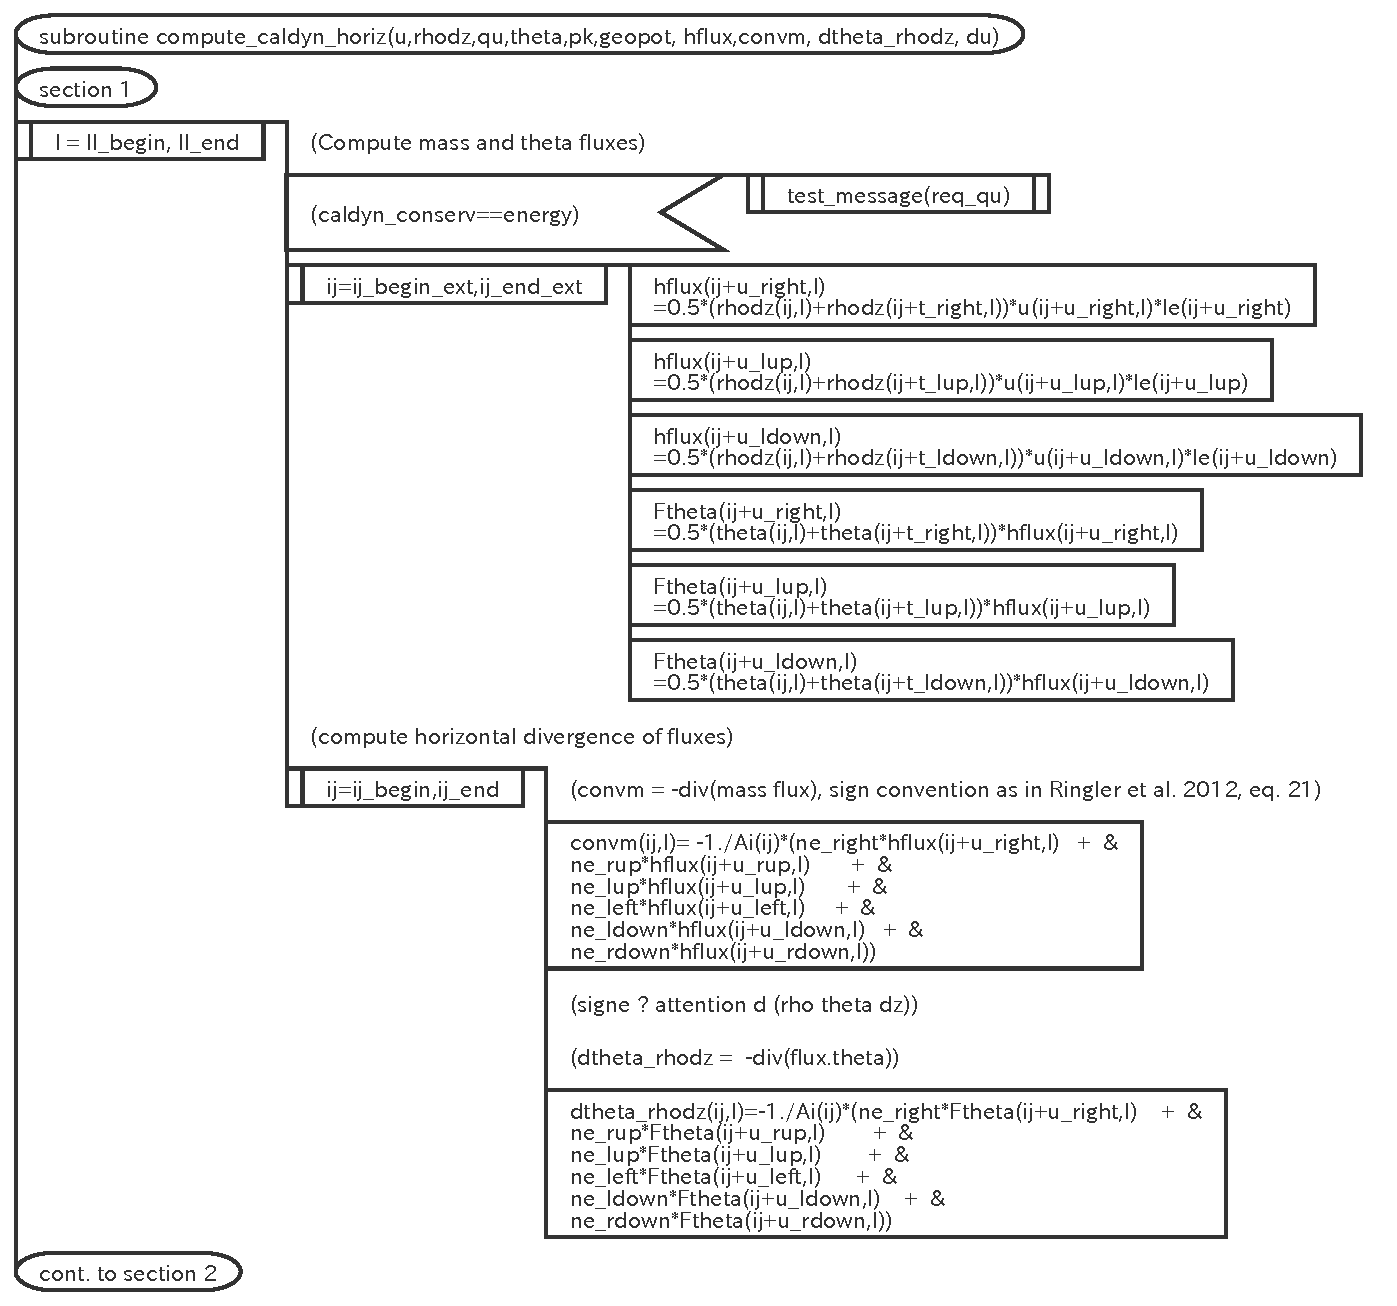
\includegraphics[scale=.6]{figs/caldyn_horiz_sec1.pdf}
 \caption{PAD of \src{compute_caldyn_horiz(1)}}\label{f:pad_comp_caldyn_horiz_1}
\end{figure}


The second section (\autoref{f:pad_comp_caldyn_horiz_2}) calculates potential
vorticity contribution to \src{du} based on the TRiSK scheme
\citep{Ringler:2010:UAE:1749635.1750220}.
%
Here \src{wee} is interpolating weight, prepared in module
\src{geometry} in original \DYNAMICO.
%
Note that since \src{caldyn_conserv} is set as
\src{energy} in this kernel program, second choice of CASE is selected.


\begin{figure}[tbp]
\centering
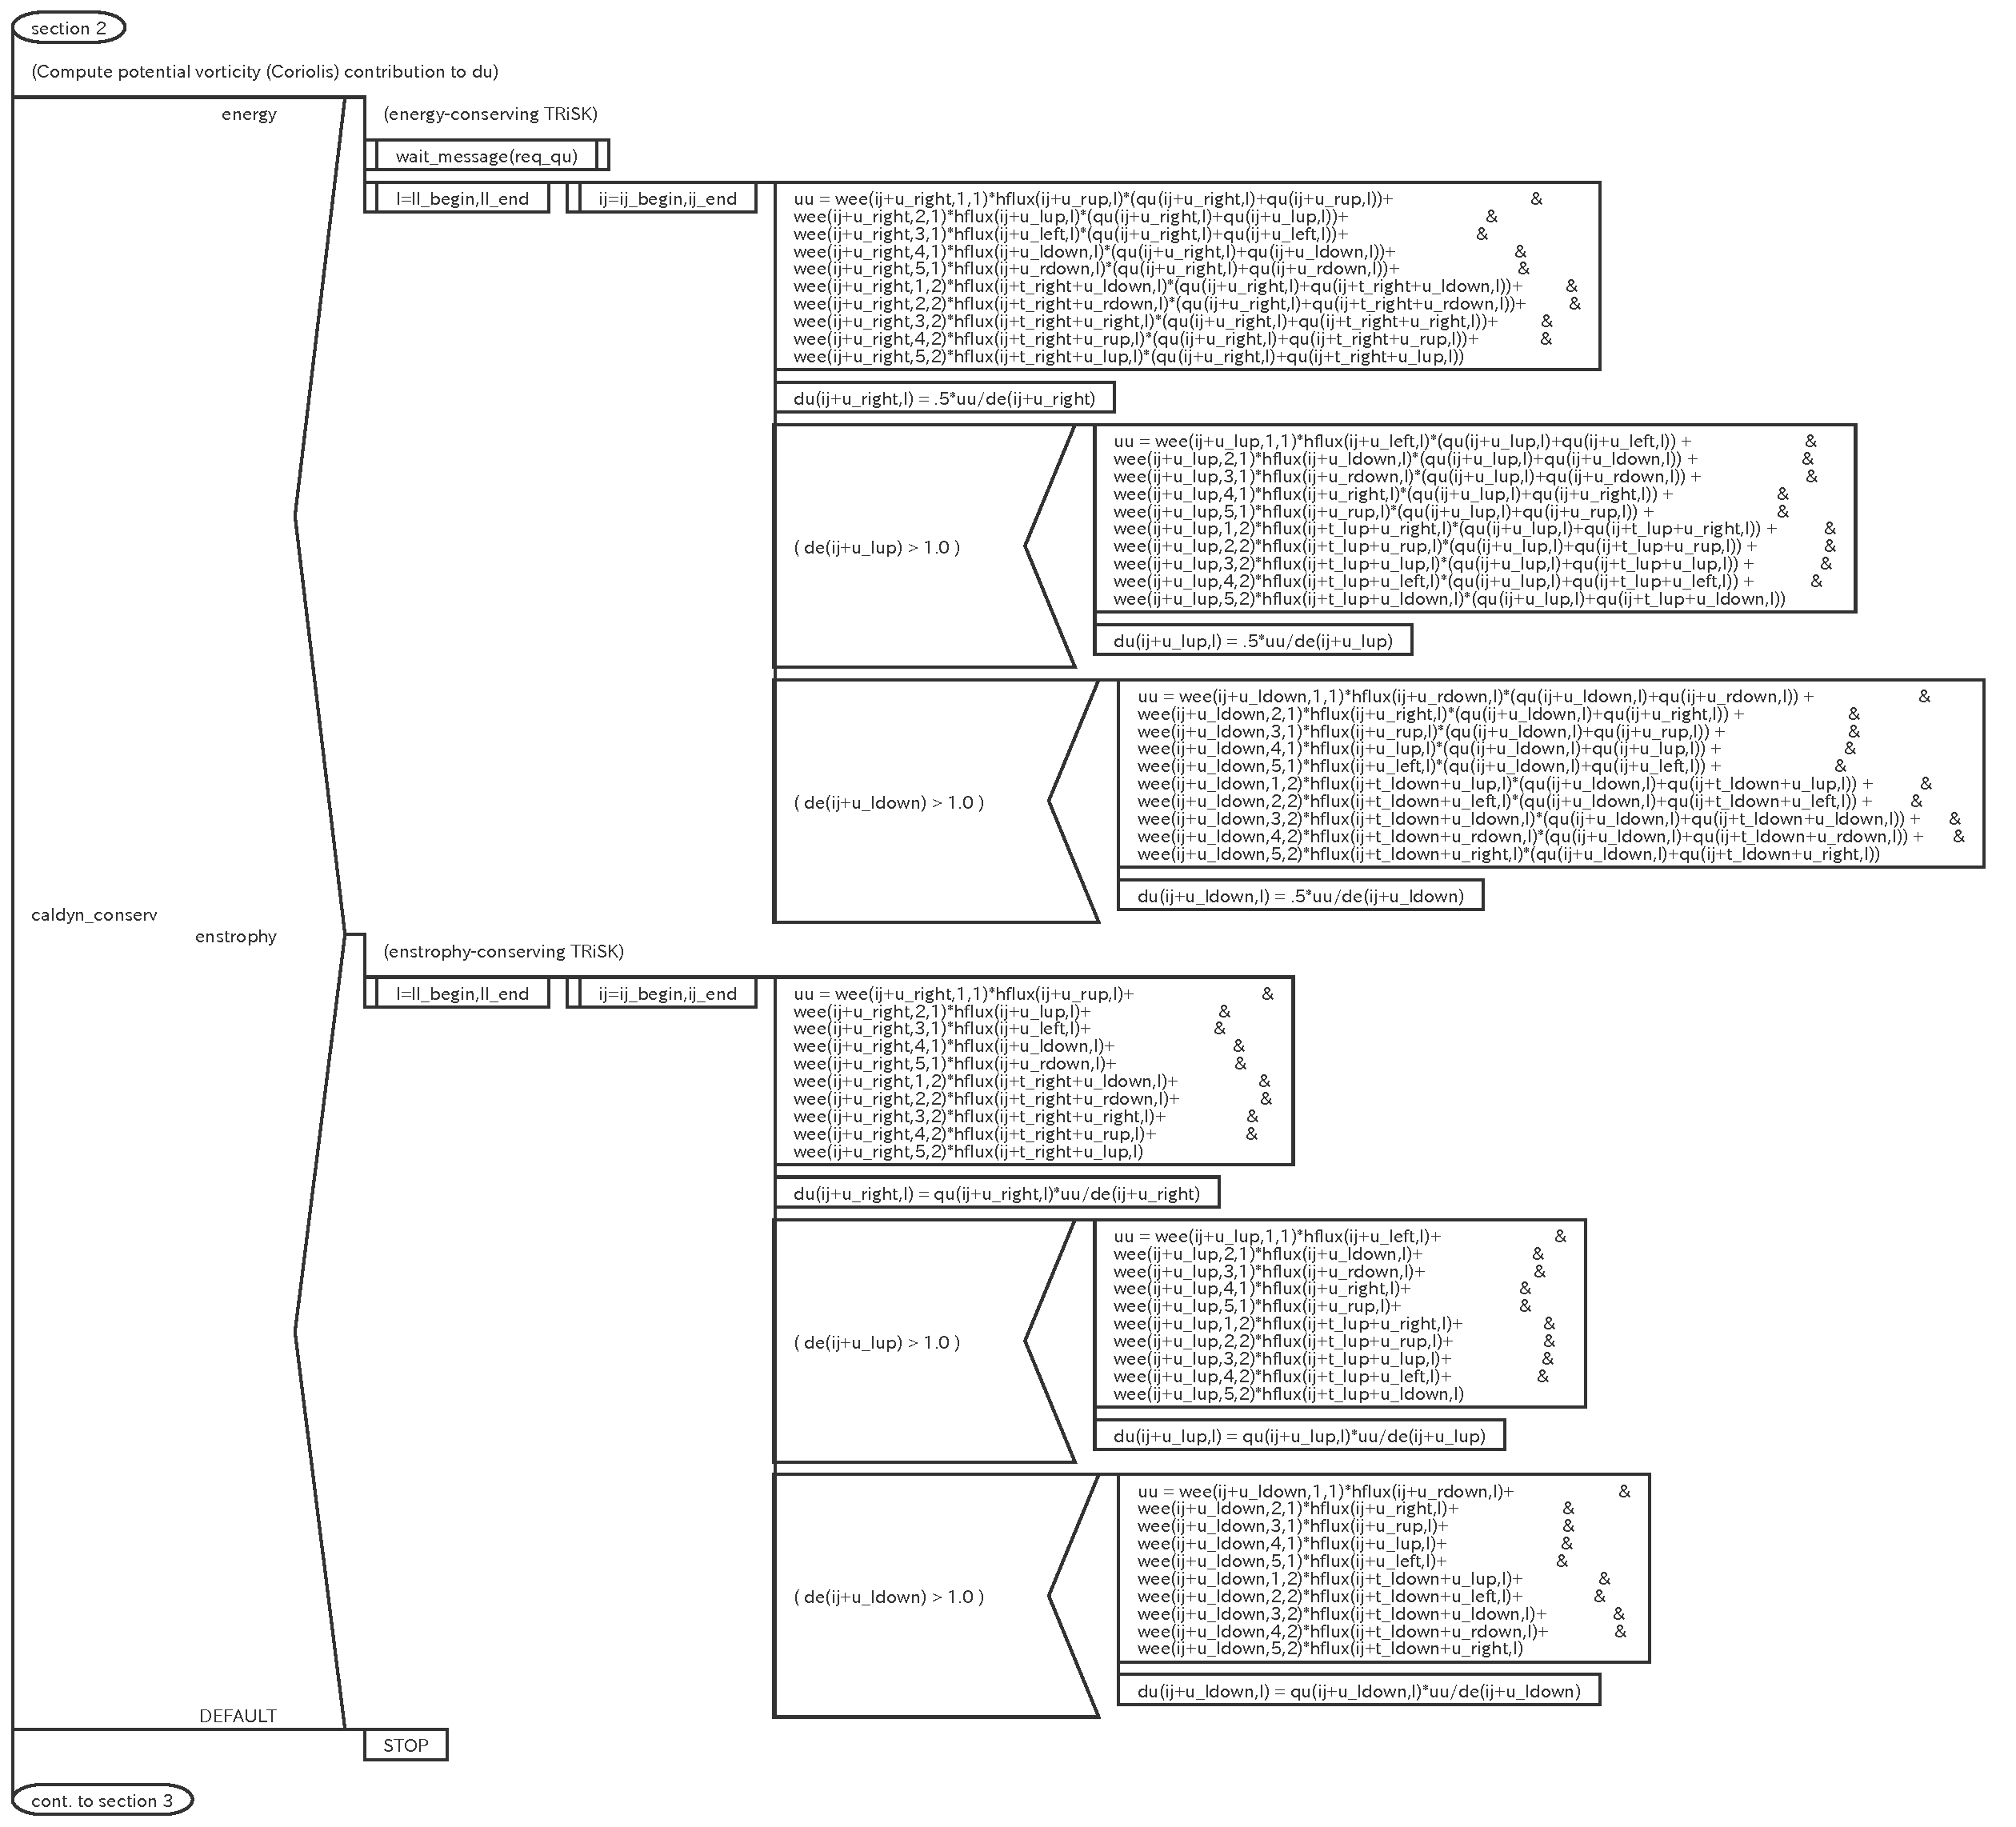
\includegraphics[scale=.4]{figs/caldyn_horiz_sec2.pdf}
 \caption{PAD of \src{compute_caldyn_horiz(2)}}\label{f:pad_comp_caldyn_horiz_2}
\end{figure}

The last section (\autoref{f:pad_comp_caldyn_horiz_3}) calculates Bernoulli term
first, then adds gradients of it and Extern functions to \src{du}.
%
Here Bernoulli term is sum of kinetic energy and geopotential.
%
Note that \src{boussinesq} is set as \src{.true.} in this kernel
package, Exner function \src{pk} is calculated in advance to calculate
Bernoulli term \src{berni}.

\begin{figure}[tbp]
\centering
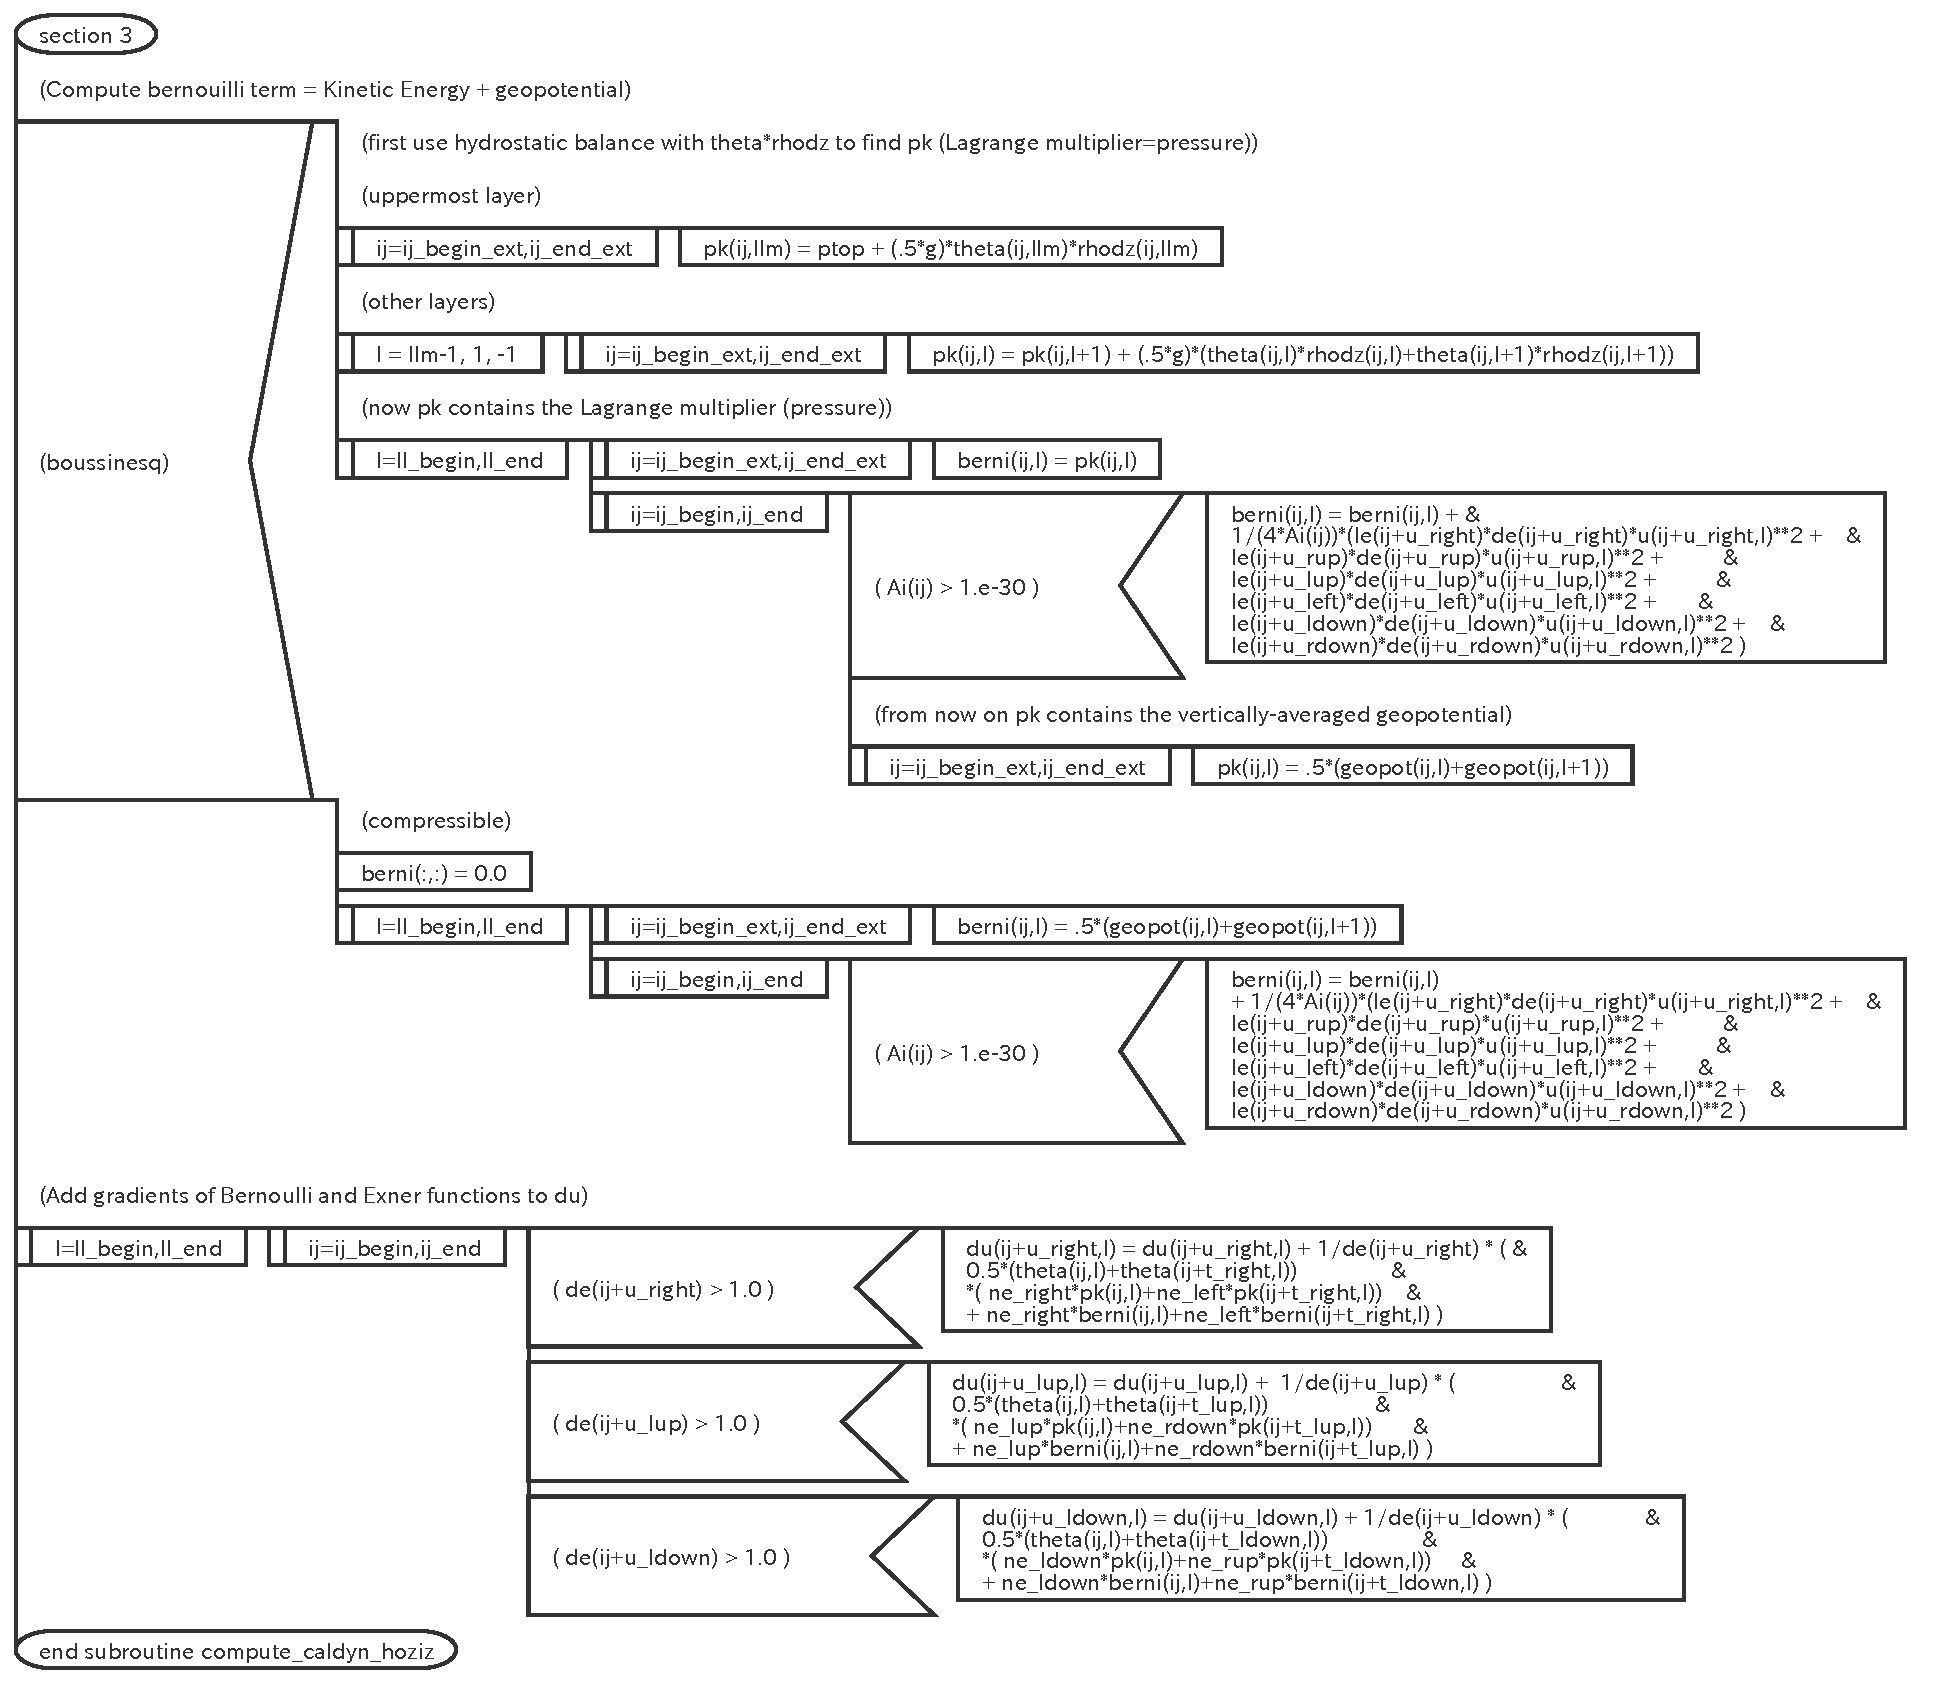
\includegraphics[scale=.5]{figs/caldyn_horiz_sec3.pdf}
 \caption{PAD of \src{compute_caldyn_horiz(3)}}\label{f:pad_comp_caldyn_horiz_3}
\end{figure}

\clearpage


\subsection{Input data and result}

Input data file is prepared and you can download from official server using
\file{data/download.sh} script.
%
This data file is created by original \DYNAMICO\footnotemark with
Held-Suarez case parameter set included in the original source archive.
%
\footnotetext{with slight modification by AICS.}
%
Max/min/sum of input/output data of the kernel subroutine are output as
a log.
%
Below is an example of \src{$IAB_SYS=Ubuntu-gnu-ompi} case.

\begin{LstLog}
 [KERNEL] comp_caldyn_horiz
 *** Start  initialize
                iim, jjm, llm:    23    25    19
             ij_begin, ij_end:    48   528
     ij_begin_ext, ij_end_ext:    24   552
             ll_begin, ll_end:     1    19
        t_right, t_rup, t_lup:     1    23    22
     t_left, t_ldown, t_rdown:    -1   -23   -22
        u_right, u_rup, u_lup:     0  1173   575
     u_left, u_ldown, u_rdown:    -1  1150   553
           z_rup, z_up, z_lup:   598     0   597
     z_ldown, z_down, z_rdown:   -23   575   -22
               caldyn_conserv:     1
                   boussinesq:     F
                            g:     9.80000000
 +check[pk_prev         ] max=  1.0014594722514462E+03,min=  0.0000000000000000E+00,sum=  6.9872296819747351E+06
 +check[hflux_prev      ] max=  0.0000000000000000E+00,min=  0.0000000000000000E+00,sum=  0.0000000000000000E+00
 +check[convm_prev      ] max=  0.0000000000000000E+00,min=  0.0000000000000000E+00,sum=  0.0000000000000000E+00
 +check[dtheta_rhodz_pre] max=  0.0000000000000000E+00,min=  0.0000000000000000E+00,sum=  0.0000000000000000E+00
 +check[du_prev         ] max=  3.4399140149818440E-03,min= -3.0658810374294527E-03,sum=  5.5109794763703335E-01
 +check[le              ] max=  1.3457165724385556E+05,min=  0.0000000000000000E+00,sum=  1.6031419146648201E+08
 +check[Ai              ] max=  3.4618288017294556E+10,min=  0.0000000000000000E+00,sum=  1.7746401564746273E+13
 +check[de              ] max=  4.5171816240714993E+06,min=  0.0000000000000000E+00,sum=  4.7785815753077912E+08
 +check[Av              ] max=  4.1228713627140027E+11,min=  0.0000000000000000E+00,sum=  3.2428753277257527E+13
 +check[Wee             ] max=  5.9893054722291683E-01,min= -5.8540209553487599E-01,sum=  2.4695023837951297E+01
 *** Finish initialize
 *** Start kernel
 ### check point iteration:           1
 ### Input ###
 +check[u               ] max=  4.1278968179782127E-01,min= -4.1278968179782127E-01,sum=  1.6791131703073393E+01
 +check[rhodz           ] max=  1.2306877011993038E+03,min=  0.0000000000000000E+00,sum=  5.3979591836733194E+06
 +check[qu              ] max=  1.0339537867296609E-06,min= -8.4408169682701225E-07,sum=  3.9419811615778674E-04
 +check[theta           ] max=  8.0139914420291746E+02,min=  0.0000000000000000E+00,sum=  3.8582633571973117E+06
 +check[geopot          ] max=  3.8250620498369227E+05,min=  0.0000000000000000E+00,sum=  1.1718001851963627E+09
 +check[pk_prev         ] max=  1.0014594722514462E+03,min=  0.0000000000000000E+00,sum=  6.9872296819747351E+06
 +check[hflux_prev      ] max=  0.0000000000000000E+00,min=  0.0000000000000000E+00,sum=  0.0000000000000000E+00
 +check[convm_prev      ] max=  0.0000000000000000E+00,min=  0.0000000000000000E+00,sum=  0.0000000000000000E+00
 +check[dtheta_rhodz_pre] max=  0.0000000000000000E+00,min=  0.0000000000000000E+00,sum=  0.0000000000000000E+00
 +check[du_prev         ] max=  3.4399140149818440E-03,min= -3.0658810374294527E-03,sum=  5.5109794763703335E-01
 ### Output ###
 +check[pk              ] max=  1.0014594722514462E+03,min=  0.0000000000000000E+00,sum=  6.9872296819747351E+06
 +check[hflux           ] max=  3.1805763161244854E+07,min= -2.8604204589892026E+07,sum=  2.4131331333014986E+08
 +check[convm           ] max=  1.0361970643226587E-03,min= -1.0359249303947807E-04,sum= -1.5233533963107249E-01
 +check[dtheta_rhodz    ] max=  3.2251351666935379E-01,min= -3.3676276308628725E-02,sum= -5.3720539414185993E+01
 +check[du              ] max=  3.4404317002518906E-03,min= -3.0804630348046005E-03,sum=  5.5048589972605033E-01
 ### final iteration:        1000
 ### Validation : grid-by-grid diff ###
 +check[pk              ] max=  0.0000000000000000E+00,min=  0.0000000000000000E+00,sum=  0.0000000000000000E+00
 +check[hflux           ] max=  0.0000000000000000E+00,min=  0.0000000000000000E+00,sum=  0.0000000000000000E+00
 +check[convm           ] max=  0.0000000000000000E+00,min=  0.0000000000000000E+00,sum=  0.0000000000000000E+00
 +check[dtheta_rhodz    ] max=  0.0000000000000000E+00,min=  0.0000000000000000E+00,sum=  0.0000000000000000E+00
 +check[du              ] max=  0.0000000000000000E+00,min=  0.0000000000000000E+00,sum=  0.0000000000000000E+00
 *** Finish kernel
\end{LstLog}

Check the lines below \src{``Validation : grid-by-grid diff''} line,
that shows difference between calculated output array and
pre-calculated reference array.
These should be zero or enough small to be acceptable.
%
There are sample output log files in \file{reference/}
in each kernel program directory, for reference purpose.

\subsection{Sample of performance result}

Here's an example of the performance result part of the log output.
Below is an example executed with the machine environment described in \autoref{s:measuring_env}.
%
Note that in this program kernel part is iterated 1000 times.

\begin{LstLog}
 *** Computational Time Report
 *** ID=001 : MAIN_comp_caldyn_horiz           T=     0.876 N=   1000
\end{LstLog}

\section{\src{comp_caldyn_vert}}

\subsection{Description}

Kernel \src{comp_caldyn_vert} is taken from the original subroutine
\src{compute_caldyn_vert} in \DYNAMICO.
%
This subroutine is originally defined in module \src{caldyn_gcm_mod}.
%
This module defines subroutine \src{caldyn}, which is the main
subroutines for dynamics part of the model, and several sub-subroutines
for various terms in the governing equation, such as potential
vorticity, geopotential, etc.
%
This subroutine calculates vertical mass flux and vertical transport.



\subsection{Discretization and code}


\autoref{l:definition_comp_caldyn_vert} shows the definition part of this subroutine,
and \autoref{f:pad_comp_caldyn_vert} shows the PAD of this.


\begin{LstF90}[%
caption={Definition part of \src{compute_caldyn_vert}},%
label={l:definition_comp_caldyn_vert}%
]
SUBROUTINE compute_caldyn_vert(u,theta,rhodz,convm, wflux,wwuu, dps,dtheta_rhodz,du)
  USE icosa
  USE disvert_mod
  USE exner_mod
  USE trace
  USE omp_para
  IMPLICIT NONE
    REAL(rstd),INTENT(IN)  :: u(iim*3*jjm,llm)
    REAL(rstd),INTENT(IN)  :: theta(iim*jjm,llm)
    REAL(rstd),INTENT(IN)  :: rhodz(iim*jjm,llm)
    REAL(rstd),INTENT(INOUT)  :: convm(iim*jjm,llm)  ! mass flux convergence

    REAL(rstd),INTENT(INOUT) :: wflux(iim*jjm,llm+1) ! vertical mass flux (kg/m2/s)
    REAL(rstd),INTENT(INOUT) :: wwuu(iim*3*jjm,llm+1)
    REAL(rstd),INTENT(INOUT) :: du(iim*3*jjm,llm)
    REAL(rstd),INTENT(INOUT) :: dtheta_rhodz(iim*jjm,llm)
    REAL(rstd),INTENT(INOUT) :: dps(iim*jjm)

! temporary variable
    INTEGER :: i,j,ij,l
    REAL(rstd) :: p_ik, exner_ik
    INTEGER,SAVE ::ij_omp_begin, ij_omp_end
!$OMP THREADPRIVATE(ij_omp_begin, ij_omp_end)
    LOGICAL,SAVE :: first=.TRUE.
!$OMP THREADPRIVATE(first)
\end{LstF90}
%
Where \src{u}, \src{theta}, \src{rhodz} are wind velocity on the edge,
potential temperature, and mass, respectively.
\src{convm}, \src{wflux}, \src{wwuu} are mass flux convergence, vertical mass flux,
and \src{wflux*u} on the edge, respectively.
%
Last three variables are time derivatives.
\src{du}, \src{dtheta_rhodz}, \src{dps} are for wind velocity on the edge,
mass-weighted potential temperature, and surface pressure, respectively.
%
All of these except \src{dps} are two dimensional.
%
First dimension is for horizontal index, and the size depends on the
point where the variable is defined, since \DYNAMICO adopts C-grid.
%
Second dimension is for vertical index, and the size is \src{llm},
except \src{llm+1} for \src{wflux} and \src{wwuu}, these are defined on
the half level in vertical, while others are defined on the full level.

\begin{figure}[tbp]
 \centering
 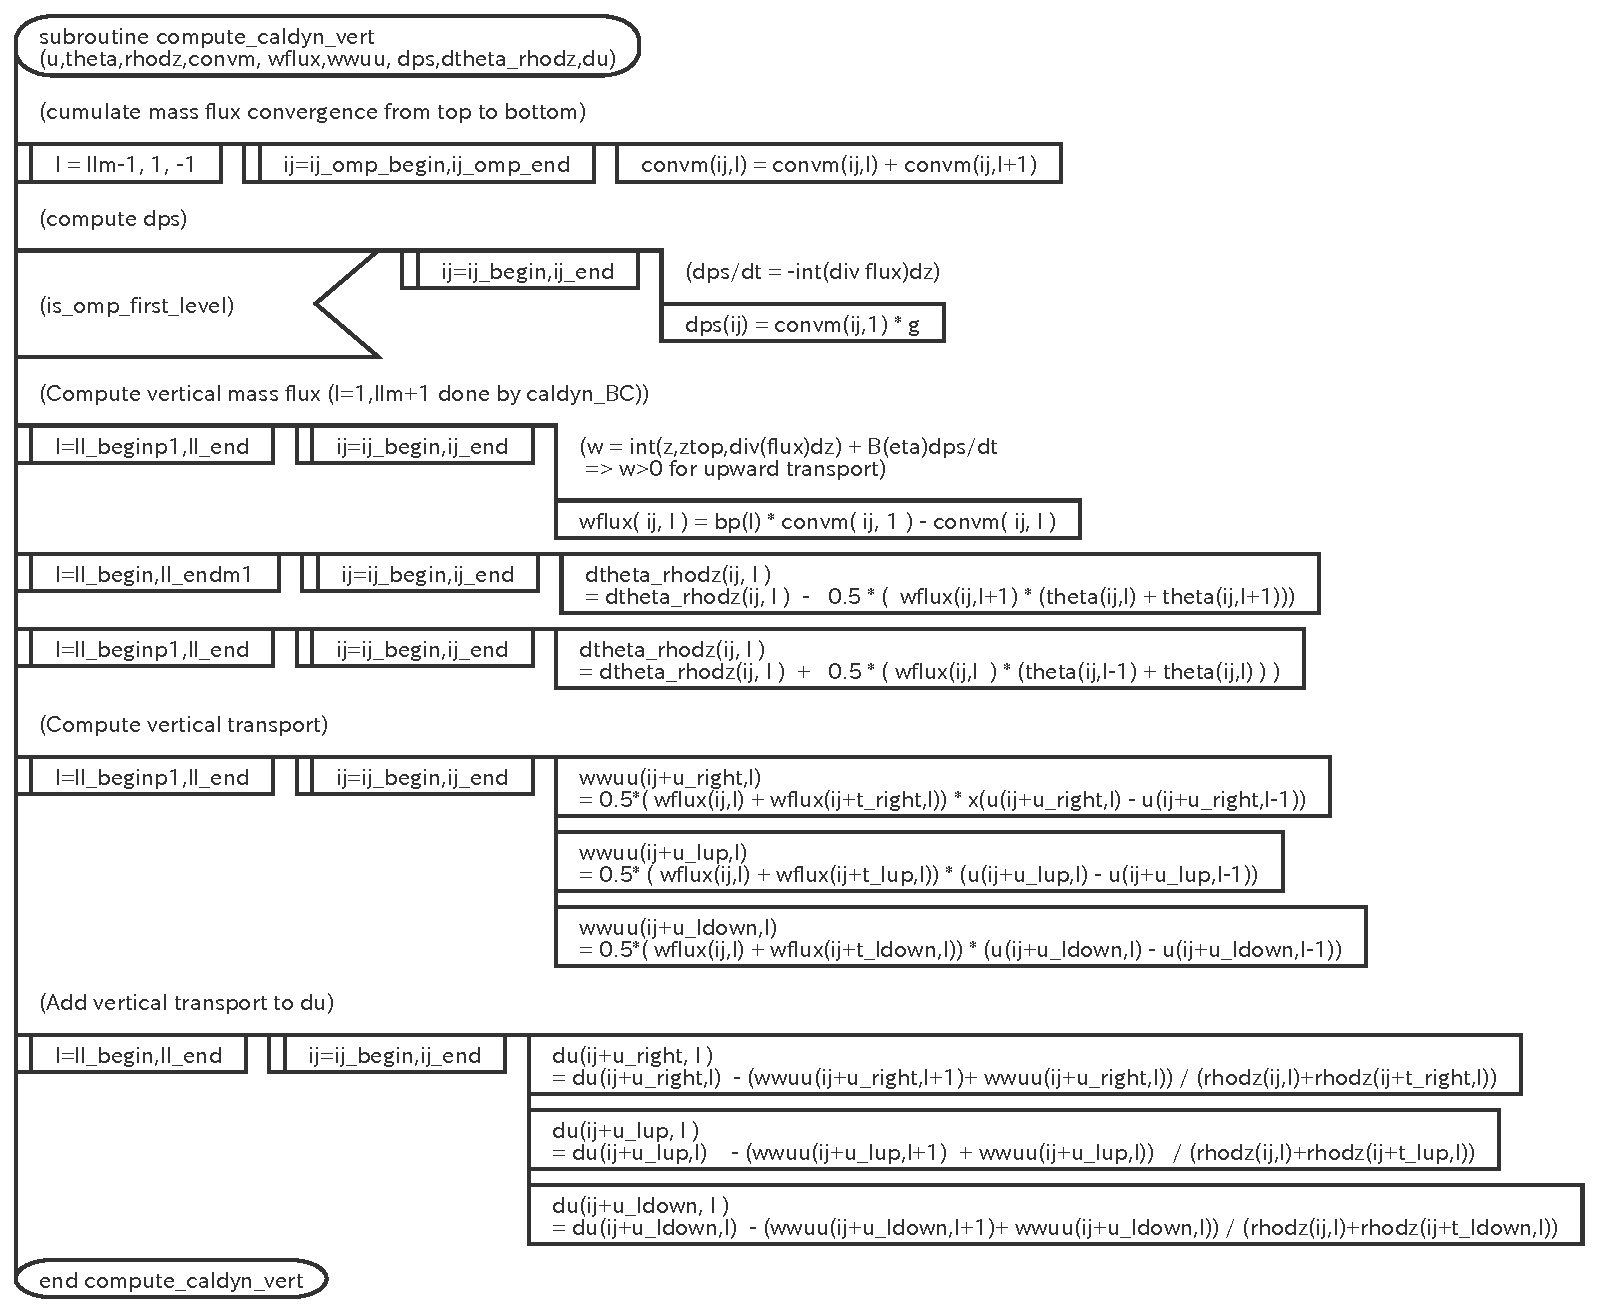
\includegraphics[scale=.5]{figs/caldyn_vert.pdf}
 \caption{PAD of \src{compute_caldyn_vert}}
 \label{f:pad_comp_caldyn_vert}
\end{figure}

Main part of this subroutine is consist of several $l$- and $ij$- double loop.
%
The first double loop is to accumulate mass flux convergence from top to bottom,
then convert \src{convm} at the lowest level to \src{dps}.
%
The second double loop is to compute vertical mass flux \src{wflux}.
%
Note that the range of $l$-loop, because \src{wflux} is defined on half
vertical level and at the top and the bottom are already set by
subroutine \src{caldyn_BC} as a boundary condition.
%
Next two double loop is to calculate convergence of potential
temperature \src{dtheta_rhodz}.
%
Again note that the range of two $l$-loop, since \src{dtheta_rhodz} is
defined on full vertical level and needs to sum up both upper and lower
face of the level.
%
Next two double loop is to compute vertical transport \src{wwuu}, and to
add it to \src{du}.
%
Note the horizontal index here.
%
\src{wwuu} and \src{du} are defined on the edge
of control volume, there are three statement in each double loop.

\clearpage



\subsection{Inputdata and result}

Input data file is prepared and you can download from official server using
\file{data/download.sh} script.
%
This data file is created by original \DYNAMICO\footnotemark with
Held-Suarez case parameter set included in the original source archive.
%
\footnotetext{with slight modification by AICS.}
%
Max/min/sum of input/output data of the kernel subroutine are output as
a log.
%
Below is an example of \src{$IAB_SYS=Ubuntu-gnu-ompi} case.

\begin{LstLog}
 [KERNEL] comp_caldyn_vert
 *** Start  initialize
                iim, jjm, llm:    23    25    19
             ij_begin, ij_end:    48   528
     ij_begin_ext, ij_end_ext:    24   552
             ll_begin, ll_end:     1    19
         ll_beginp1, ll_endm1:     2    18
        t_right, t_rup, t_lup:     1    23    22
     t_left, t_ldown, t_rdown:    -1   -23   -22
        u_right, u_rup, u_lup:     0  1173   575
     u_left, u_ldown, u_rdown:    -1  1150   553
           z_rup, z_up, z_lup:   598     0   597
     z_ldown, z_down, z_rdown:   -23   575   -22
                       dbg: g:     9.80000000
 +check[bp              ] max=  1.0000000000000000E+00,min=  0.0000000000000000E+00,sum=  6.9254510678414132E+00
 *** Finish initialize
 *** Start kernel
 ### check point iteration:        1000
 ### Input ###
 +check[u               ] max=  4.1278968179782127E-01,min= -4.1278968179782127E-01,sum=  1.6791131703073393E+01
 +check[theta           ] max=  8.0139914420291746E+02,min=  0.0000000000000000E+00,sum=  3.8582633571973117E+06
 +check[rhodz           ] max=  1.2306877011993038E+03,min=  0.0000000000000000E+00,sum=  5.3979591836733194E+06
 +check[convm_prev      ] max=  1.0361970643226587E-03,min= -1.0359249303947807E-04,sum= -1.5233533963107249E-01
 +check[wflux_prev      ] max=  0.0000000000000000E+00,min=  0.0000000000000000E+00,sum=  0.0000000000000000E+00
 +check[wwuu_prev       ] max=  0.0000000000000000E+00,min=  0.0000000000000000E+00,sum=  0.0000000000000000E+00
 +check[du_prev         ] max=  3.4404317002518906E-03,min= -3.0804630348046005E-03,sum=  5.5048589972605033E-01
 +check[dtheta_rhodz_pre] max=  3.2251351666935379E-01,min= -3.3676276308628725E-02,sum= -5.3720539414185993E+01
 +check[dps_prev        ] max=  0.0000000000000000E+00,min=  0.0000000000000000E+00,sum=  0.0000000000000000E+00
 ### Output ###
 +check[convm           ] max=  6.9593389571287302E-03,min= -7.9269107622801825E-04,sum= -1.5227927267389074E+00
 +check[wflux           ] max=  4.1171035230973149E-04,min= -3.6145630748324665E-03,sum=  5.8901163077820706E-01
 +check[wwuu            ] max=  1.7149300599654128E-04,min= -1.8768192515764522E-04,sum= -5.0377733672629036E-04
 +check[du              ] max=  3.4404317002518906E-03,min= -3.0804630348046005E-03,sum=  5.5048632410110032E-01
 +check[dtheta_rhodz    ] max=  3.5427038431326496E-01,min= -4.2032604085394595E-02,sum= -5.3720539414186263E+01
 +check[dps             ] max=  6.8201521779861565E-02,min= -7.7683725470345790E-03,sum= -1.3213658793877174E+00
 ### final iteration:        1000
 ### Validation : grid-by-grid diff ###
 +check[convm           ] max=  0.0000000000000000E+00,min=  0.0000000000000000E+00,sum=  0.0000000000000000E+00
 +check[wflux           ] max=  0.0000000000000000E+00,min=  0.0000000000000000E+00,sum=  0.0000000000000000E+00
 +check[wwuu            ] max=  0.0000000000000000E+00,min=  0.0000000000000000E+00,sum=  0.0000000000000000E+00
 +check[du              ] max=  0.0000000000000000E+00,min=  0.0000000000000000E+00,sum=  0.0000000000000000E+00
 +check[dtheta_rhodz    ] max=  0.0000000000000000E+00,min=  0.0000000000000000E+00,sum=  0.0000000000000000E+00
 +check[dps             ] max=  0.0000000000000000E+00,min=  0.0000000000000000E+00,sum=  0.0000000000000000E+00
 *** Finish kernel
\end{LstLog}

Check the lines below \src{``Validation : grid-by-grid diff''} line,
that shows difference between calculated output array and
pre-calculated reference array.
These should be zero or enough small to be acceptable.
%
There are sample output log files in \file{reference/}
in each kernel program directory, for reference purpose.

\subsection{Sample of performance result}

Here's an example of the performance result part of the log output.
Below is an example executed with the machine environment described in \autoref{s:measuring_env}.
%
Note that in this program kernel part is iterated 1000 times.

\begin{LstLog}
 *** Computational Time Report
 *** ID=001 : MAIN_comp_caldyn_vert            T=     0.156 N=   1000
\end{LstLog}




\bibliographystyle{plainnat}
\bibliography{reference}

\appendix
\chapter{Brief description of PAD}\label{s:pad}

\section{PAD is }

Problem Analysis Diagram (PAD) is to describe the logical structure of
the program by the two dimensional tree.
%
PAD is suitable for structured programing, like Fortran.




\section{Elements in PAD}

In PAD, one box shows one process or one sentence in Fortran, and
only three basic structure is allowed; sequence, conditional branch, and iteration.

\subsection{Sequence}

%
Simple sequence of sentence is shown as listed box in same vertical line
from top to bottom
(\autoref{f:pad_sequence}).
%
Subroutine call is shown as \autoref{f:pad_call}.


\begin{figure}[htbp]
\begin{minipage}{.49\textwidth}
\center
 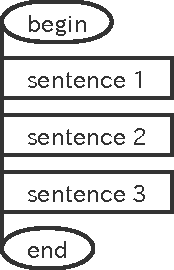
\includegraphics[scale=0.7]{figs/pad_sequence.pdf}
\end{minipage}
\begin{minipage}{.49\textwidth}
\begin{LstF90}[numbers=none]
 sentence 1
 sentence 2
 sentence 3
\end{LstF90}
\end{minipage}
\caption{elements of PAD: sequence}
\label{f:pad_sequence}
\end{figure}


\begin{figure}[htbp]
\begin{minipage}{.49\textwidth}
 \center
  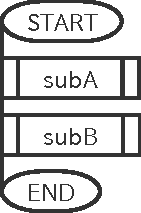
\includegraphics[scale=0.7]{figs/pad_routinecall.pdf}
\end{minipage}
\begin{minipage}{.49\textwidth}
\begin{LstF90}[numbers=none]
 call subA()
 call subB()
\end{LstF90}
\end{minipage}
 \caption{elements of PAD: subroutine call}
 \label{f:pad_call}
\end{figure}

\subsection{Conditional branch}

Conditional branch and selection are shown in the same manner.
\autoref{f:pad_if} shows the IF-THEN-ELSE type branch, and
\autoref{f:pad_case} shows the CASE type branch.

\begin{figure}[htbp]
\begin{minipage}{.49\textwidth}
 \center
  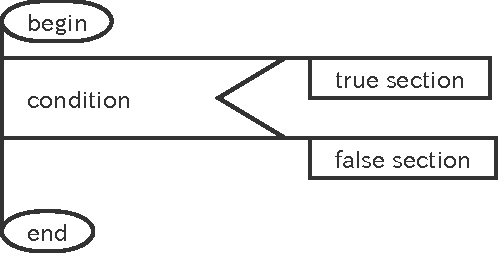
\includegraphics[scale=0.7]{figs/pad_ifelse.pdf}
\end{minipage}
\begin{minipage}{.49\textwidth}
\begin{LstF90}[numbers=none]
 if ( condition ) then
   true section
 else
   false section
 end if
\end{LstF90}
\end{minipage}
\caption{elements of PAD: IF-THEN-ELSE}
\label{f:pad_if}
\end{figure}

\begin{figure}[htbp]
\begin{minipage}{.6\textwidth}
 \center
  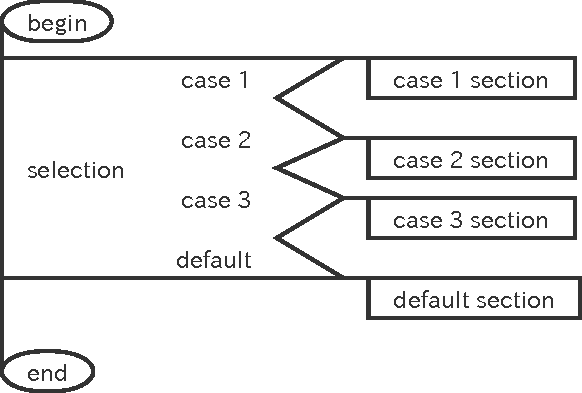
\includegraphics[scale=0.7]{figs/pad_selection.pdf}
\end{minipage}
\begin{minipage}{.4\textwidth}
\begin{LstF90}[numbers=none]
 select case ( selection )
 case (case1)
   case1 section
 case (case2)
   case2 section
 case (case3)
   case3 section
 case default
   default section
 end case
\end{LstF90}
\end{minipage}
\caption{elements of PAD: CASE Selection}
\label{f:pad_case}
\end{figure}

\subsection{Iteration}

Iteration is shown as \autoref{f:pad_iteration}.

\begin{figure}[htbp]
\begin{minipage}{.49\textwidth}
 \center
  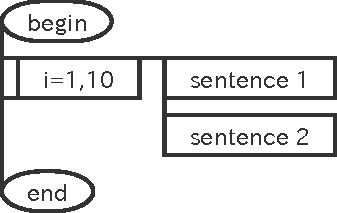
\includegraphics[scale=0.7]{figs/pad_iteration.pdf}
\end{minipage}
\begin{minipage}{.49\textwidth}
\begin{LstF90}[numbers=none]
 do i=1, 10
   sentence 1
   sentence 2
 end do
\end{LstF90}
\end{minipage}
\caption{elements of PAD: Iteration}
\label{f:pad_iteration}
\end{figure}


\subsection{Hierarchy}

Hierarchy in program is expressed as connection of boxes in right
direction.
%
So width of the PAD means complexity of the program and height means the
size of the program.
%
\autoref{f:pad_hierarcy} shows the example of hierarcy in PAD.
%
The first half shows combination of IF-THEN-ELSE clause and DO-loop, the
latter half shows usual double Do-loop.

\begin{figure}[htbp]
\begin{minipage}{.7\textwidth}
 \center
  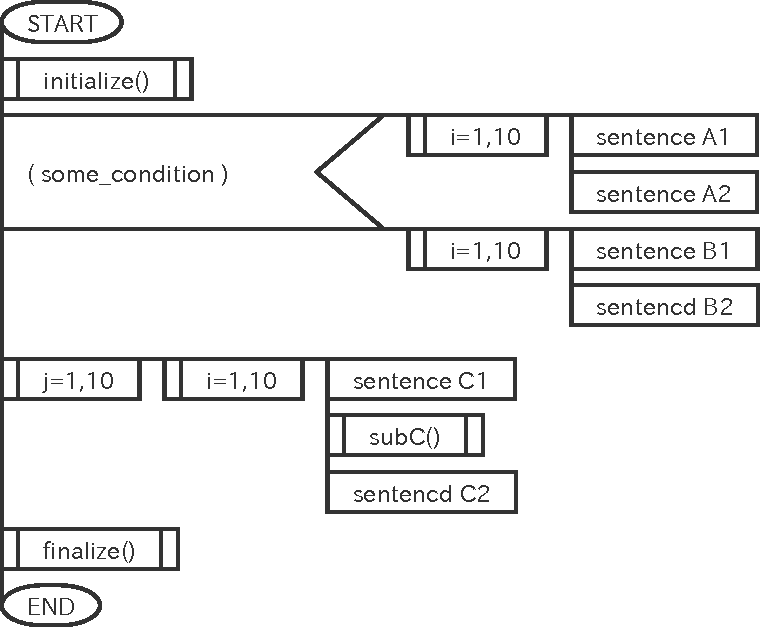
\includegraphics[scale=0.7]{figs/pad_hierarcy.pdf}
\end{minipage}
\begin{minipage}{.29\textwidth}
\begin{LstF90}[numbers=none]
 call initialize()

 if ( some_condition ) then
   do i=1,10
     sentence A1
     sentence A2
   end do
 else
   do i=1,10
     sentence B1
     sentence B2
   end do
 end if

 do j=1,10
   do i=1,10
     sentence C1
     call subC()
     sentence C2
   end do
 end do

 call finalize()
\end{LstF90}
\end{minipage}
\caption{Example of hierarcy in PAD}
\label{f:pad_hierarcy}
\end{figure}


\cleardoublepage

%====================================================================================
% Back Matter
%====================================================================================
\newpage
\thispagestyle{empty}

\mbox{\hspace*{1em}}\\

\vspace{10mm}
{\large{\bfseries IcoAtmosBenchmark NICAM kernels}}\\

\vspace{10mm}
{\large{\bfseries Author \& Editor}}\\
\hrule width 90mm
\begin{tabbing}
SPPEXA/AIMES Benchmarking team\\
\end{tabbing}


\vspace{110mm}

\begin{flushright}
\ovalbox{ \begin{minipage}{80mm}
 \noindent\small\rmfamily contact : Hisashi Yashiro (RIKEN) \src{h.yashiro@riken.jp}
\end{minipage}
}\\
\end{flushright}

\vspace{10mm}

\begin{flushright}
Copyright \copyright RIKEN, 2017-2018. All rights reserved.
\end{flushright}

%====================================================================================


\end{document}
